\documentclass[dissertation]{aaltoseries}
%\documentclass[dissertation,draft*]{aaltoseries}
%\documentclass[draft]{aaltoseries}
%\usepackage{aaltothesis}
\usepackage[utf8]{inputenc}
%\usepackage[utf8]{fontenc}
%\usepackage{pslatex}
%\usepackage{ae,aecompl}
\usepackage[T1]{fontenc}
\usepackage[finnish,english]{babel}
\usepackage{lipsum}
%\usepackage{auto-pst-pdf}
%\usepackage{amssymb}
%\usepackage{amsmath}
\usepackage{url}
\usepackage{psfrag,color,pstricks,pst-grad}
\usepackage[normalem]{ulem}
%\usepackage{graphicx}
%\usepackage[pdftex]{graphicx}
%\usepackage{lipsum}% just to automatically generate text
\usepackage{amsmath,amsfonts,amssymb,amsbsy}  
\usepackage{hyperref}
\usepackage{enumitem}
\usepackage{upgreek}
\usepackage{siunitx}
\usepackage{tabularx}
%\usepackage{setspace}
%\doublespacing
\newcommand{\ud}{\mathrm{d}}
\newcommand{\bb}{\mathbf}
\newcommand{\ca}{\mathcal}

\hyphenation{macro-scale nano-scale damped}

\newcommand{\fb}{\left[f_B(\omega,T)+\frac{1}{2} \right]}
\newcommand{\fbbg}{\left[f_B(\omega,\Tenv)+\frac{1}{2} \right]}
\newcommand{\fbi}{\left[f_B(\omega,T_{i})+\frac{1}{2} \right]}
\newcommand{\fbj}{\left[f_B(\omega,T_{j})+\frac{1}{2} \right]}
\newcommand{\mbb}{\mathbb}
\newcommand{\gem}{\mathbb{G}}
\newcommand{\gems}{\mathbb{g}}
\newcommand{\bu}{\bb{u}}
\newcommand{\bd}{\bb{d}}
\newcommand{\bE}{\bb{E}}
\newcommand{\br}{\bb{r}}
\newcommand{\bp}{\bb{p}}
\newcommand{\bG}{\bb{G}}
\newcommand{\Pfluc}{\bb{P}_{\textrm{fluc}}}
\newcommand{\pom}{(\omega)}
\newcommand{\epsenv}{\varepsilon_{\textrm{env}}}
\newcommand{\Tenv}{T_{\textrm{env}}}
\newcommand{\Eenv}{\bb{E}_{\textrm{env}}}
\newcommand{\Eenvhat}{\hat{\bb{E}}_{\textrm{env}}}
\newcommand{\Eenvtilde}{\tilde{\bb{E}}_{\textrm{env}}}
\newcommand{\gemfull}{{\gem}^{\textrm{CM}}}
\newcommand{\tildegemfull}{{\gem}^{\textrm{full}}}
\newcommand{\kw}{k_0}
\newcommand{\unitdyadic}{\bb{I}_{3 \times 3}}
\newcommand{\change}{\uline}
%\newcommand{\change}{}
\newcommand{\listofsymbols}{%
  \chapter*{Symbols and abbreviations}%
}


% The author of the dissertation
\author{Kimmo S\"a\"askilahti}
% The title of the thesis


\title{Computational modeling and spectral\\ analysis of nanoscale energy transfer}

\begin{document}
% \doublespace
\pagenumbering{roman}

\draftabstract{Swift progress in the synthesis and processing of materials with nanoscale feature sizes has spawned new possibilities to control the flow of thermal energy. New materials and devices with engineered thermal properties are expected to enable, e.g., clean and more efficient production of energy from waste heat by thermoelectric converters, reducing the energy consumption of digital electronics, and generating novel technologies such as heat-assisted magnetic recording and phase-change memories. As the classical laws of energy transfer do not generally apply in nanoscale, practical realization of such applications calls for powerful computational methods delivering scientific understanding of nanoscale heat transfer.

The goal of this thesis is to develop new computational models and methods for describing energy transfer in atomic-scale structures and to apply the methods to generate useful insight into various thermal phenomena. The work is founded on classical molecular dynamics simulations and quantum-mechanical Green's function approaches, both using the fluctuation-dissipation theorem to couple the studied systems to external heat baths. To enable detailed analysis of energy transfer mechanisms in thermal conduction, new methods to spectrally decompose the lattice heat current into frequency components are also developed. Spectral analysis is applied in the thesis to identify non-linear energy transfer mechanisms at material interfaces and to determine the mean free paths of heat carriers in carbon nanotubes. The results also suggest that the thermoelectric efficiency of silicon nanowires can be increased by a specific superlattice structure and that the electromagnetic energy transfer rate between dielectric nanoparticles can be tuned by a mirror cavity.

In addition, the thesis initiates the development of a unified fluctuational model for describing energy transfer by lattice vibrations, electromagnetic fields, and electrons in a single mathematical framework that can generate extensive understanding of the energy conversion phenomena present in small structures. As a whole, the methods and results of the thesis provide new analytical and numerical tools for describing nanoscale energy transfer within a framework that may, with further development, become instrumental also in modeling energy conversion and transfer processes in multiscale systems involving heat, light and electricity.}

\draftabstract[finnish]{Nanoteknologian nopea kehitys on synnytt\"anyt uusia tapoja hallita l\"amp\"oenergiaa. L\"amp\"oenergian tehokkaan hallinnan ja ohjauksen odotetaan mahdollistavan mm. puhtaan energiantuotannon termos\"ahk\"oisill\"a materiaaleilla, digitaalielektroniikan tehonkulutuksen pienent\"amisen sek\"a t\"aysin uusien sovellusten kuten l\"amp\"oohjatun magneettisen tallentamisen kehitt\"amisen. L\"amp\"oenergiaa hy\"odynt\"avien sovellusten kehitt\"aminen vaatii kuitenkin erinomaista ymm\"arryst\"a energiansiirtomekanismeista hyvin pieniss\"a rakenteissa.

V\"ait\"oskirjaty\"on tavoitteena on kehitt\"a\"a uusia laskennallisia malleja ja menetelmi\"a l\"amm\"onsiirron mallintamiseen nanomittakaavan rakenteissa sek\"a soveltaa menetelmi\"a uuden ymm\"arryksen synnytt\"amiseen. Ty\"o perustuu klassiseen ep\"atasapainotilan molekyylidynamiikkamenetelm\"a\"an sek\"a kvanttimekaanisiin Greenin funktio -laskuihin, jotka molemmat hy\"odynt\"av\"at fluktuaatio-dissipaatioteoriaa tarkasteltavan systeemin ja ymp\"arist\"on v\"alisen kytkenn\"an kuvaamiseen. L\"amm\"onjohtumismekanismien analysoimiseksi kehitet\"a\"an mm. menetelm\"a hilav\"ar\"ahtelyjen kuljettaman l\"amp\"ovirran jakamiseksi taajuuskomponentteihin. Ty\"on malleja ja spektraalista hajotelmaa sovelletaan ep\"alineaaristen l\"amm\"onsiirtomekanismien tunnistamiseen materiaalirajapinnoilla sek\"a l\"amp\"o\"a kuljettavien hilav\"ar\"ahtelyjen sirontapituuksien m\"a\"aritt\"amiseen hiilinanoputkissa. Ty\"on tulokset osoittavat my\"os, ett\"a piinanolankojen termos\"ahk\"oisi\"a ominaisuuksia voidaan parantaa erityisell\"a superhilarakenteella ja ett\"a s\"ahk\"omagneettisen l\"amm\"onsiirron voimakkuutta nanopartikkeleiden v\"alill\"a voidaan muokata sijoittamalla partikkelit peilikaviteettiin.

Ty\"oss\"a kehitet\"a\"an lis\"aksi yhten\"ainen matemaattinen malli hilav\"ar\"ahtelyjen, s\"ahk\"omagneettisten kenttien ja elektronien l\"amm\"onkuljetuksen mallintamiseen. Kokonaisuudessaan v\"ait\"oskirjaty\"o tarjoaa energiansiirron mallintamiseen ty\"okaluja, jotka voivat tulevaisuudessa olla merkitt\"av\"ass\"a roolissa valon, s\"ahk\"on ja l\"amm\"on vuorovaikutuksien kuvaamisessa eri mittakaavan rakenteissa.}

% 

\author{Kimmo S\"a\"askilahti}
\begin{preface}[Espoo, Finland]
Preface text
\end{preface}

\vspace{1cm}
\noindent
\textit{Funding organizations, computational resources}

\tableofcontents

\listofpublications

\chapter*{Summary of article contents}
\addcontentsline{toc}{chapter}{Summary of article contents}

\textbf{Publication I} investigates the role of anharmonic phonon scattering in thermal conduction across planar material interfaces and provides the first application of the spectral decomposition formula for heat current. The results show that anharmonic phonon scattering facilitates thermal conduction across the interface by providing a dissipation mechanism for evanescent waves and by enabling multi-phonon energy transfer processes at the interface.

\vspace{1cm}
\noindent
\textbf{Publication II} presents a new method for determining the frequency-dependent phonon mean free paths from non-equilibrium simulations. The determined mean free paths directly reflect the decay of heat current in non-equilibrium, allowing for straightforwardly assessing the contributions of different vibrational frequencies to thermal conduction in tubes of different lengths. Room-temperature mean free paths in carbon nanotubes are shown to exceed 10 $\upmu$m at low frequencies, highlighting their extraordinary thermal properties with applications in, e.g., thermal management of electronics. 

\vspace{1cm}
\noindent
\textbf{Publication III} presents the first study of the effect of periodic twinning stacking faults on the thermal conductivity of silicon nanowires. Molecular dynamics simulations show that the nanowire thermal conductivity can be notably reduced by the periodic twinning, suggesting the possibility to increase the thermoelectric efficiency by such superlattice structures.

\vspace{1cm}
\noindent
\textbf{Publications IV, V} and \textbf{VI} focus on thermal conduction in nanoscale point contacts. Simulations for point contacts in a two-dimensional square lattice reveal interference patterns in local temperature profiles, not captured by Fourier's law. Quantum statistics are shown to modify temperature profiles in point contacts at low temperatures, but the effect is shown to be weak for graphene at room temperature.

\vspace{1cm}
\noindent
\textbf{Publication VII} presents Langevin theory of electromagnetic energy transfer, providing an alternative description complementing the traditional fluctuational electrodynamics. Numerical results for nanoparticles in a mirror cavity demonstrate the possibility to tune the rate of electromagnetic energy transfer between dielectric bodies by an inhomogeneous environment, in analogy to the well-known Purcell effect enabling the tuning of spontaneous emission.

\chapter*{Author's contribution}
\addcontentsline{toc}{chapter}{Author's contribution}
The author wrote the first draft, developed and/or adapted the required theoretical and numerical models and performed all the calculations and numerical analysis in \textbf{Publications I, II, IV, V, VI}, and \textbf{VII}.

\vspace{1cm}
\noindent
The author actively contributed to the writing of the manuscript and participated in the interpretation of numerical results in \textbf{Publication III}.

\listofsymbols
\addcontentsline{toc}{chapter}{Symbols and abbreviations}
\setlist[description]{style=multiline,topsep=10pt,leftmargin=3cm,font=\normalfont\normalfont\space,align=parleft}

\begin{description} \itemsep2pt
  \item[$\alpha^{\textrm{CM}}$] Clausius-Mossotti polarizability
  \item[$c$] Electron annihilation operator 
  \item[$c^{\dagger}$] Electron creation operator 
  \item[$C$] Position autocorrelation function
  \item[$d$] Dipolar displacement 
  \item[$\delta_{ij}$] Kronecker delta
   \item[$\delta(x-x')$] Dirac delta function
  \item[$\Delta T$] Temperature difference
  \item[$D$] Nanowire diameter
    \item[$e$] Local vibrational energy
   \item[$E$] Electric field  
   \item[$E_{\textrm{env}}$] Background electric field
   \item[$\varepsilon$] Electric permittivity
   \item[$\varepsilon_0$] Vacuum permittivity
   \item[$\varepsilon_{\textrm{env}}$] Electric permittivity of the environment
   \item[$\eta$] Electron Langevin noise operator
   \item[$f$] Frequency
   \item[$f_{\textrm{BE}}$] Bose-Einstein function
   \item[$f_{\textrm{FD}}$] Fermi-Dirac function
  \item[$F$] Force
   \item[FDT] Fluctuation-dissipation theorem
  \item[$g$] Spectrally decomposed thermal conductance
  \item[$G$] Green's function matrix
  \item[$\mathbb{G}$] Electromagnetic Green's dyadic
  \item[GF] Green's function 
  \item[$\gamma$] Langevin friction constant
  \item[$\gamma_e$] Electron Langevin friction constant
  \item[$\Gamma$] Bath coupling function
  \item[$\hbar$] Reduced Planck's constant
  \item[$H$] Magnetic field 
  \item[$\mathcal{H}_\textrm{ph}$] Lattice Hamiltonian
  \item[$\mathcal{H}_\textrm{el}$] Electron Hamiltonian
  \item[$\mathcal{H}_\textrm{el}^{\textrm{tb}}$] Electron tight-binding Hamiltonian
  \item[$\bb{I}_{3\times 3}$] $3\times 3$ unit matrix
  \item[$j$] Polarization current
  \item[$k_B$] Boltzmann constant
  \item[$K$] Force constant matrix 
   \item[$\lambda_{\textrm{max}}$] Thermal wavelength
  \item[$\Lambda$] Phonon mean free path
  \item[$L$] System length
  \item[$L_{\textrm{bath}}$] Length of heat bath
   \item[$\mu$] Chemical potential
  \item[$\mu_0$] Vacuum permeability
  \item[$m$] Mass of atom or dipole
  \item[$m_e$] Electron mass
  \item[MD] Molecular dynamics
  \item[$n$] Refractive index
  \item[$N$] Number of atoms
  \item[NEMD] Non-equilibrium molecular dynamics
  \item[$\xi$] Langevin force 
  \item[$\omega$] Angular frequency
  \item[$\omega_0$] Oscillator resonance frequency
  \item[$\omega_r$] Phonon-polariton resonance frequency
    \item[$p$] Dipole moment
  \item[$p^{\textrm{kin}}$] Kinetic momentum  
  \item[$P$] Electric polarization density
  \item[$P_{\textrm{ind}}$] Induced part of electric polarization density
  \item[$P_{\textrm{fluc}}$] Fluctuating part of electric polarization density
  \item[$\phi$] Localized electron eigenstate
  \item[$q$] Dipole charge
  \item[$q(\omega)$] Spectral decomposition of heat current
  \item[$Q$] Heat current
  \item[$Q^{\textrm{bath}}$] Heat current to bath
  \item[$r$] Atom position
  \item[$r_0$] Equilibrium position of atom 
  \item[$R$] Nanoparticle radius
   \item[$\Sigma$] Bath self-energy
  \item[$\sigma$] Electron orbital index
  \item[$S$] Poynting vector
  \item[$t$] Time
  \item[$t_{ij}^{\sigma\sigma'}$] Electron tight-binding hopping constant
  \item[$T$] Temperature
  \item[$T_D$] Debye temperature
  \item[$\mathcal{T}$] Transmission function
  \item[$u$] Displacement of atom from equilibrium position
  \item[$\Upsilon$] Anharmonic force constant
  \item[${V}$] Electron potential energy
  \item[$\mathcal{V}$] Interatomic potential energy function
  \item[$W$] System width
  % \item[$\bu_i$] Vector displacement of atom $i$ 
  \item[$\chi$] Electric susceptibility
\end{description}

\chapter{Introduction}
\setcounter{page}{1}
\pagenumbering{arabic}
%\chapter{Introduction}
\label{chap:intro}
\section{Motivation}

Significant advancements in the fields of micro and nanotechnology in recent decades have enabled the engineering of new materials with improved electrical, thermal and optical properties \cite{}. This miniaturization has drawn considerable attention into thermal effects, which are crucial for, e.g., designing more efficient thermoelectrics \cite{vineis10,kanatzidis10,shakouri11} and tackling the problem of overheating in microprocessors \cite{pop06_ieee}. Thermal effects play the main role also in completely new technologies such as phase-change memory \cite{lankhorst05}, heat-assisted magnetic recording \cite{pan09}, tumor therapy based on nanoparticle laser heating \cite{avedisian09}, and information processing using temperature \cite{li12_rmp}. For all such applications, a solid understanding of energy transfer processes in nanoscale is necessary. %To tackle the power problem and to enable efficient thermal engineering, thorough understanding of heat transfer mechanisms are required. 
%  temperature-related 

% Nanoscale physics richer in nanoscale

Theoretically, energy is transferred in solid-state systems by lattice vibrations, electromagnetic fields, and electrons \cite{chen}. Compared to macroscale, where thermal transfer is often characterized by a few constitutive material parameters, heat transfer in nanoscale is enriched by the presence of various length scales comparable to the system size \cite{chen}. As a consequence, classical heat transfer laws such as Fourier's law of conduction \cite{fourier} and Planck's law of radiation \cite{planck00a} break down, giving rise to exotic phenomena such as thermal conductance quantization \cite{rego98,schwab00} and monochromatic thermal radiation \cite{carminati99,shchegrov00}. In addition, the microscopic coupling of energy carriers in nanoscale can prohibit their separate treatment and require unified models accounting for energy conversion from one form to other. 

% Accounting for such phenomena requires sophisticated models. Second, microscopic coupling of energy carriers in nanostructures prohibits their separate treatment as in macroscale. For example, the smooth transition from radiation-dominated energy transfer at large material separations to vibration-dominated at small separations was only recently described theoretically by including both electromagnetic fields and lattice vibrations in a single model \cite{xiong14,chiloyan15}. 

\textbf{One more binding paragraph before the objectives...}

\section{Scope and objectives}
% Smooth transition to scope and objectives, explain how different carriers play together at small scales
% Mapping of possibilities
% New computational methods
% Combining phononic, photonic and eventually electronic transport into a single model

This doctoral thesis aims at creating physical insight into heat transfer in nanoscale systems by atomic scale simulations accompanied by the development of new computational tools and methods. The main focus areas of the thesis are (i) modeling energy transfer by phonons \footnote{Throughout the thesis, we refer to lattice vibrations loosely as phonons, which are the quanta of normal mode oscillations \cite{ziman}.} in various geometries using classical methods, and (ii) developing quantum-mechanical computational methods for describing vibrational, electromagnetic as well as electronic energy transfer in a single theoretical framework to eventually enable the combination of the models. In all our studies, we only consider solid state systems, thereby excluding convection from the considered list of energy transfer mechanisms. %We limit our scope to heat transfer by lattice vibrations and electromagnetic radiation, thereby excluding both electronic conduction and convection.

For the first focus area, we employed classical molecular dynamics simulations to model lattice heat transfer in different systems. While MD neglects quantum effects, it can flexibly account for atomic-scale geometries, wave interference effects and so-called anharmonic scattering between lattice waves. Using MD, we answer the following questions: 
 \begin{itemize}
  \item How does anharmonic scattering manifest in energy transfer at material interfaces?
  \item What role do interference and dissipative effects play in thermal conduction through nanoscale point contacts smaller than phonon wavelength and mean free path?
  \item How far can phonons travel in carbon nanotubes without being damped by anharmonic scattering?
  \item How does so-called twinning affect the thermal conductivity of silicon nanowires?
 \end{itemize}

% \begin{itemize}
%   \item Anharmonic scattering assists energy transfer between dissimilar materials by (i) enabling dissipation of evanescent waves and (ii) allowing for multi-phonon energy transfer across the interface
% \end{itemize}

In the second area of focus, we pave the way for the unified theoretical description of phononic, photonic (electromagnetic) and electronic energy transfer. We show that Langevin theory \cite{langevin,zwanzig} combined with the linearization of equations of motion allows for calculating energy transfer rates for the three primary carriers in a unified manner, fully accounting for both wave properties and carrier relaxation and also allowing for simulations of relatively large systems. Since such a unified mathematical picture of energy transfer for the three carriers has not been presented earlier, this compilation part of the thesis is taken as an opportunity to highlight the opportunities presented by such a treatment.

To put these research topics in the general context of nanoscale heat transfer, we briefly review the most prominent nanoscale energy transfer phenomena below and also discuss the structures investigated in each of the publications included in this thesis. Detailed theory and methods are presented in Chap. \ref{chap:theory}. Highlights from the results are presented in Chap. \ref{chap:results}.

% The two focus areas listed above roughly divide the publications included in this thesis into two parts. First part of the thesis is devoted to lattice vibrations (loosely referred to as phonons), because they are the dominant heat transfer mechanism in insulators and typical semiconductors \cite{chen}. To deliver new insight into phononic energy transfer processes, we use classical molecular dynamics (MD) simulations. While MD neglects all quantum effects, it accounts both for wave interference and detailed scattering phonon scattering without any approximations \footnote{Except for assuming classical wave dynamics and employing a semi-empirical potential for describing interatomic interactions.}. Using MD, we investigate the following questions:
% \begin{itemize}
%  \item Does the interplay of interference and dissipative effects manifest in structures smaller than phonon wavelength and mean free path?
%  \item What is the role of anharmonic effects in energy transfer at material interfaces?
%  \item What are the limits of ballistic heat transfer in low-dimensional structures such as carbon nanotubes?
% \end{itemize}

%(1) study how interference and anharmonic scattering manifest in thermal transfer through a point contact, (2) investigate the detailed role of anharmonic scattering in energy transfer across a planar interface between two materials of different masses, and (3) calculate phonon scattering lengths in carbon nanotubes from non-equilibrium MD simulations, and (4) demonstrate tunable thermal conductivity in twinning superlattice silicon nanowires.

% In the second part, we pave the way for the unified theoretical description of phononic, photonic and electronic energy transfer.
% \begin{itemize}
%  \item Is there a unified way to describe energy transfer of phonons, photons, and electrons using simple computational models?
% \end{itemize}
% Our results show that Langevin theory \cite{langevin,zwanzig} combined with the linearization of equations of motion allows fo calculating energy transfer rates for the three primary carriers in a unified manner, fully accounting for both wave properties and carrier relaxation and also allowing for simulations of relatively large systems. Since such a unified, mathematical picture of energy transfer for the three carriers cannot be found in literature, this compilation part of the thesis is taken as an opportunity to highlight the opportunities presented by such a treatment.

% The solution of the Langevin equations of motion naturally gives rise to Green's functions, which act as response functions translating local stochastic fluctuations in carrier number into carrier propagation. Dissipative effects are mimicked by the coupling of the microscopic degrees of freedom such as atomic displacement or local dipole moment to the Langevin baths, giving rise to non-zero carrier relaxation times.




%\begin{itemize}
% \item Interference, particles versus waves
% \item Boundaries and interfaces
% \item Ballistic versus diffusive, coherence
%\end{itemize}


\section{Energy transfer in nanoscale systems}
%\begin{itemize}
% \item Phonon, photon, electron transport overlap
%\end{itemize}
Nanoscale phenomena in phonon, photon and electron transport are discussed separately below. Electronic transport is not considered in any of the publications included in this thesis but is included in this compilation part to highlight the similarities in the theoretical description of different carriers and to provide the basis for possible future works aiming at the coupling of models. Therefore, the discussion of electron transport only considers the electron-phonon and electron-photon interactions.  % Therefore, the discussion of electronic effects is kept brief throughout.  

% We begin with vibrational energy transfer phenomena in Subsection \ref{sec:intro_vib}. Emphasis is placed on the microscale violations of the classical Fourier's heat equation \cite{fetter}
% \begin{equation}
%  \rho c_p \frac{\partial T(\mathbf{r},t)}{\partial t} =  \nabla \cdot [\kappa \nabla T(\mathbf{r},t)] + q(\mathbf{r},t), \label{eq:fourier}
% \end{equation}
% which accurately describes energy transfer in macroscopic media. In Eq. \eqref{eq:fourier}, $\rho$ is mass density, $c_p$ is the constant-pressure heat capacity per unit mass, $T(\mathbf{r},t)$ is local temperature at position $\mathbf{r}$ at time $t$, $\kappa$ is the sum of electronic and phononic thermal conductivities and $q(\mathbf{r},t)$ is the rate of heat generated by, e.g., Joule heating. Section. \ref{sec:intro_vib} defines the various length scales emerging in the microscopic scale, relevant in understanding when Fourier's heat equation can be safely applied. 

% Electromagnetic energy transfer phenomena in nanoscale are discussed in Subsection \ref{sec:intro_em}. In electromagnetic energy transfer, the macroscopic laws of thermal radiation such as Planck's radiation law break down when the separation between bodies becomes similar to the wavelengths of thermally excited electromagnetic fields. At such small separations, evanescent near-fields localized close to the material surfaces can couple the materials and thereby strongly increase energy transfer rates. 

% Subsection \ref{sec:intro_electrons} reviews the problem of self-heating in electronic devices. The discussion of electron transport is included in this compilation part of the thesis only to suggest a unified framework for modeling electron, phonon, and photon transport and, e.g., electron-phonon energy transfer, so the review is kept brief. Detailed electron transport topics such as the microscopic calculation of carrier scattering rates \cite{ziman} are outside the scope of this thesis.  % electron conductance quantization \cite{landauer57} and 

% Finally, Subsection \ref{sec:intro_coupling} is devoted to discussing the interplay of carriers at nanoscale, relevant to understanding, e.g., heat transfer at metal-dielectric interfaces, heat spreading in laser heating, and radiation-conduction crossover at vacuum-gaps.

% Hot spots
% Graphene quilts etc.
% Measurement of thermal conductivity from Joule heating 
% Conductance at metal-dielectric interfaces
% Current induced forces?

% Similarity of phonon, photon systems (interference, scattering, Green's function methods,...)

\subsection{Phononic thermal conduction in nanoscale}
\label{sec:intro_vib}
% Start from Peierls's theory
% \begin{itemize}
%  \item Size effects: boundaries, interfaces
%  \item Reduction of thermal conductivity (twinning nanowires)
%  \item Ballistic thermal conduction in carbon nanotubes
%  \item Wave interferences (phononic crystals, two-path interference,\dots)
% \end{itemize}



As conjenctured by Debye in 1914 \cite{}, heat is carried in semiconductors and insulators\footnote{In metals and heavily doped semiconductors, the electronic contribution often overwhelms the phononic contribution to thermal conductivity.} by propagating lattice waves called phonons. The resistance to heat flow arises microscopically from the scattering of phonons from material impurities, interfaces, and boundaries as well as other phonons and charge carriers \cite{peierls29,ziman}. These scattering mechanisms are depicted in Fig. \ref{fig:intro_scattering}. 

\begin{figure}
\begin{center}
 %\includegraphics[width=8.6cm]{pics/schwab00_fig3.ps}
 \includegraphics[width=.99\columnwidth]{inkscape/scattering.pdf}
 \caption{(a) Schematic illustration of microscopic scattering mechanisms in phononic thermal conduction: (1) Boundary scattering, (2) interface scattering, (3) phonon-phonon scattering. (b) Schematic of phonon propagation in a material, with scattering events at averages distances of mean free path $\Lambda$. \textbf{SCHEMATIC TO BE FINISHED, PERHAPS DRAW IN 2D FOR CLARITY}}
\label{fig:intro_scattering}
\end{center}
\end{figure}

The characteristic distance between phonon scattering events is called the phonon mean free path. While phonon mean free paths depend strongly on the material, temperature, and the type of scattering (elastic versus inelastic), a typical value for bulk silicon is around $\sim 300$ nm at room temperature \cite{ju99}. At length scales smaller than the mean free path, scattering events are too infrequent to drive phonon gas to local thermal equilibrium. Consequently, the classical Fourier's law of diffusion \cite{fourier} based on the concept of a well-defined local temperature breaks down. 

Because of the relatively long intrinsic phonon mean free paths and the high surface-to-volume ratio typical to nanostructures, material interfaces and surfaces often have a dominant contribution to thermal resistance. Microscopically, phonon scattering at the interface between dissimilar materials arises both from atomic disorder at the interface and from the mismatch in the acoustic properties of the materials \cite{}. Thermal resistance at interfaces can prevent the efficient extraction of heat from electronic devices, thereby limiting their performance \cite{pop10}. Many methods have been suggested to reduce the thermal resistance between materials, including chemical functionalization \cite{hopkins11,kaur14}, external pressure \cite{shen11,chalopin12}, and heat-mediating thin films \cite{english12}. 

In a similar way, boundary scattering from material surfaces can strongly reduce the thermal conductivity in nanowires and thin films. Because such reduction is expected to increase the thermoelectric figure of merit \cite{chen}, low-dimensional materials such as silicon nanowires have been suggested to be attractive alternatives for thermoelectric conversion \cite{hochbaum08}. To reduce the thermal conductivity of nanowires even further, one can apply other thermal conductivity reduction mechanisms such as alloying \cite{} or partial amorphization \cite{}. % , but with care so that electrical conduction is not too strongly hindered. % depicted in Fig. \ref{fig:intro_hochbaum}. %\citepub{spectral}\citepub{twinning} % The diffusive scattering from the atomically rough surfaces reduces the thermal conductivity of silicon nanowires by two orders of magnitude compared to the bulk value  \cite{hochbaum08}.

Efficient extraction of heat from electronic devices requires not only small interfacial resistances but also bulk materials with high thermal conductivities \cite{pop10}. Nanomaterials with long phonon mean free paths have been suggested to be good candidates for such thermal management. For example, the rigid sp$^2$ bonding of carbon atoms in carbon nanotubes \cite{iijima91} gives rise to a thermal conductivity in the range of 500-5000 W/mK \cite{}. Because of the very long mean free paths, however, the measured thermal conductivities depend on the tube length \cite{chang08}, with size-dependent variations observed even in millimeter-long nanotubes \cite{chang_personal}. It is even possible that the thermal conductivity of pristine carbon nanotubes diverges as a function of tube length, a signature of anomalous thermal conduction observed in computer simulations for one-dimensional atomic chains \cite{lepri03,mai07,dhar08}. Indications of anomalous thermal conduction were recently observed experimentally \cite{xu14} for graphene \cite{}, the two-dimensional allotrope of carbon.

% Classical heat equation \eqref{eq:fourier} follows from the conservation of energy accompanied by Fourier's law of diffusion \cite{fourier}
% \begin{equation}
%  \mathbf{q} = -\kappa \nabla T(\mathbf{r},t),
% \end{equation}
% stating that local heat flux $\bb{q}$ is proportional to the negative temperature gradient. Fourier's law is built on the assumption that the local temperature $T(\bf{r},t)$ can be sensibly defined. Because temperature is a statistical quantity properly defined only for large systems \cite{}, the law must break down at small enough length scales. 

% The microscopic theory of thermal conduction was developed by Rudolf Peierls in 1929 \cite{peierls29}. Understanding that collective lattice vibrations (phonons) carry heat in crystalline solids, he proposed that thermal resistivity arises from the scattering of phonons from lattice imperfections and other phonons. These scattering mechanisms existing in any non-ideal material at non-zero temperature give rise to a finite phonon mean free path, characterizing the average distance between scattering events. At length scales much larger than the mean free path, the heat carriers are expected to essentially perform a random walk with constant drift along the temperature gradient and heat transfer is well described by Fourier's local theory. At length scales smaller than the mean free path, on the other hand, phonons can travel without scattering and Fourier's theory must be invalid. Phonon mean free paths depend strongly on the material, vibrational frequency and temperature \cite{}, but a typical value for bulk silicon is around $\sim 300$ nm at room temperature \cite{ju99}. 

% Thermal conduction in macroscopic systems is traditionally described using Fourier's law \cite{fourier}, stating that the heat flux at any given point is proportional to the temperature gradient at the same point. The theory leads, however, to the unphysical phenomenon that a local temperature perturbation can propagate infinitely fast \cite{chen}, in direct contradiction to the finiteness of the speed of sound and also special relativity. This indicates that Fourier's theory must ultimately break down in nanoscale.

 %Some experiments have claimed to have observed such anomalous thermal conduction in silicon nanowires \cite{yang10}, but the evidence remains inconclusive. % In two-dimensional materials such as graphene, similar divergence is expected, and recent experiments and simulations for graphene have suggested this to be the case \cite{xu14}. %\citepub{cnt}

% \begin{figure}
% \begin{center}
%  %\includegraphics[width=8.6cm]{pics/schwab00_fig3.ps}
%  \includegraphics[width=8.6cm]{pics/schwab_fig3.pdf}
%  \caption{Thermal conductance measured as a function of temperature by Schwab \textit{et al.} \cite{schwab00}. In their experimental setup, heat was transferred through four nanowires with four acoustic modes in each carrying the heat. The measured conductance at low temperature is therefore $G=16g_0$, where $g_0$ is the conductance quantum. Reprinted with permission from Ref. \cite{schwab00}.}
% \label{fig:intro_schwab}
% \end{center}
% \end{figure}

% In systems smaller than the phonon mean free path, the scattering-free propagation of phonons is called ballistic transport, contrasting with the diffusive transport of Fourier-like systems. The most striking example of ballistic transport is the thermal conductance quantization, predicted theoretically by Rego and Kirczenow in 1998 \cite{rego98} and observed experimentally in 2000 by Schwab \textit{et al.} \cite{schwab00} (see Fig. \ref{fig:intro_schwab}), thereby indirectly confirming also the existence of ballistic transport. 

% The thermal conductance quantum, which is analogous to the quantum of electrical conductance, is independent of any material properties and only depends on temperature and Planck's constant.  Their calculations showed that at sufficiently low temperatures, where phonon scattering is minimal and only the lowest-frequency phonon modes can be excited, thermal conductance through a narrow constriction is an integer multiple of the thermal conductance quantum. 

% As noted above, heat transfer is expected to be well described by Fourier's law in sufficiently large system. This ballistic-diffusive transition has been observed in bulk-like three-dimensional systems using computer simulations \cite{saito10}. In low-dimensional systems, on the other hand, computer simulations \cite{lepri97,lepri03,mai07,dhar08} and heat transfer experiments \cite{yang10,xu14} have indicated that the Fourier limit may never be reached. In one-dimensional oscillator chains, for example, it is now widely accepted \cite{dhar08} that the thermal conductivity diverges as a function of system length following a power-law \cite{mai07}, called anomalous thermal conduction \cite{dhar08}. It is, however, still debated \cite{marconnet13} if any physical system such as a nanowire can be treated as a one-dimensional object and could therefore exhibit the divergence.

% Nanostructure

In addition to the mean free path, there is another important length scale governing heat transfer in microscopic scale: the phonon wavelength. In bulk silicon, the characteristic wavelength of thermally excited phonons is around 10 nm at room temperature \cite{ju99}. In structures with characteristic dimensions in the range of the phonon wavelength, the wave properties of phonons cannot be neglected and interference effects appear. Interference effects have enabled, for example, designing acoustic reflectors with novel applications in phonon lasing \cite{maryam13}, enhancing the optical-mechanical coupling \cite{fainstein13}, and phonon nanocapacitors \cite{han15}. \textbf{ADD SHORT DISCUSSION OF POINT CONTACTS AS THERMAL BARIERS, PERHAPS BEGIN THE PARAGRAPH FROM POINT CONTACTS?}

% Wavelength-related effects are also exploited in thermal engineering: as an example, Kim \textit{et al.} were able to reduce the thermal conductivity of InGaAs alloy, which naturally scatters short-wavelength phonons due to point defects, by introducing nanoparticles acting as scatterers for mid-to-long-wavelength phonons \cite{kim06}. %\citepub{fpu}\citepub{fpu2}\citepub{gf} % Other examples of interference

% \begin{figure}
% \begin{center}
%  %\includegraphics[width=8.6cm]{pics/schwab00_fig3.ps}
%  \includegraphics[width=.80\columnwidth]{pics/hochbaum_fig1.pdf}
%  \caption{(a) Scanning electron microscope image of a silicon nanowire array. (b) Transmission electron microscope image of a single nanowire, showing the prominent edge roughness responsible for strong phonon scattering. The low thermal conductivity gives rise to a high thermoelectric figure of merit. The electron diffraction pattern in the inset shows that the wire single crystalline along its length. Reprinted with permission from Ref. \cite{hochbaum08}.}
% \label{fig:intro_hochbaum}
% \end{center}
% \end{figure}



% Relation to the thesis
% Concepts such as phonon interference, ballistic transport, mean free paths, and interface scattering appear throughout this thesis. In Publications \cp{fpu}, \cp{fpu2}, and \cp{gf}, we explore the interference effects exhibited in thermal conduction through nanoscale constrictions and reveal intricate interference patterns in local nonequilibrium temperature profiles. We also show how such patterns vanish at higher temperatures due to increased scattering. In Publication \cp{spectral}, we present detailed maps of the contributions of different vibrational frequencies to thermal conduction across a mass-mismatched interface, improving thereby the understanding of heat transfer mechanisms at interfaces and presenting guidelines for future thermal engineering of high-conductance interfaces. Publication \cp{cnt} presents a non-equilibrium method for determining the mean free paths of phonons in carbon nanotubes, supplying a theoretical description of the ballistic-diffusive crossover in one-dimensional systems. In Publication \cp{twinning}, we perform ''thermal engineering'' and demonstrate the existence of minimun thermal conductivity at a certain twinning period length in a silicon nanowire. The minimun arises from the maximal blocking of bulk-like scattering-free propagation of phonons through the nanowire by the periodically repeating twinning boundaries.


%As noted by Kapitza already in 1930s \cite{}, carrier scattering at interfaces between materials also gives rise to thermal resistance. Even in the absence of defects, 

% Point contacts \cite{bartsch12}

% Contact resistance is a bottleneck
% Material properties increasingly dominated by interfaces

% Interfaces

% Superlattices, phonon mirrors

% While there is convincing evidence from numerical simulations that the Fourier limit is always achieved in three-dimensional systems \cite{saito10,wang10}, this seems not to be the case in one- or two-dimensional systems. Numerical simulations \cite{lepri97,mai07} and hydrodynamical theory \cite{} suggest that the thermal conductivity in one-dimensional systems diverges in a power-law fashion as a function of system length, but clear experimental demonstration of the divergence has not been achieved so far. In two-dimensional systems, thermal conductivity is expected to diverge logarithmically \cite{}. Recent experiments claim to have observed the divergence in graphene \cite{xu14}.

%\subsection{Thermal boundary resistance}

%\subsection{Thermal engineering}

\subsection{Photonic energy transfer in the near-field}
\label{sec:intro_em}

Unlike lattice vibrations, electromagnetic fields can propagate and transfer heat even in vacuum. This phenomenon is best observed on a sunny day when the electromagnetic radiation emitted from the Sun heats the skin. Like all thermal radiation, the radiation from the Sun originates from accelerating charges. Because the electrons and nuclei in any matter undergo accelerating motion due to thermal fluctuations, all matter radiates heat like a miniature Sun. 

% While lattice vibrations cannot transfer heat without a medium, electromagnetic fields can propagate even in vacuum. Because all materials emit electromagnetic radiation due to the microscopic fluctuations of electrons and nuclei, 

\begin{figure}
\begin{center}
 %\includegraphics[width=8.6cm]{pics/schwab00_fig3.ps}
 \includegraphics[width=.80\columnwidth]{inkscape/thermal_radiation.pdf}
 \caption{Due to microscopic thermal fluctuations, an object at non-zero temperature emits thermal radiation in the form of propagating electromagnetic waves (red). Close to the object, there are, however, also evanescent waves (orange) with zero propagation velocity. If another object is placed in the near-field, the contribution of evanescent waves to energy transfer between the bodies can dominate over the propagating wave contribution. \textbf{SCHEMATIC TO BE FINISHED}}
\label{fig:intro_em}
\end{center}
\end{figure}

Thermal radiation emitted from an object typically contains a wide range of photon wavelengths, with the distribution governed by the Planck distribution \cite{planck00a} and the wavelength-dependent emissivity of the object \cite{}. For objects at room temperature, the wavelength of emitted propagating waves are typically in the micrometer-range \cite{}. At distances smaller than the dominant wavelength from the object, there are, however, also evanescent waves localized close to the object as depicted in Fig. \ref{fig:intro_em}. While these evanescent waves are ''invisible'' and cannot carry energy far from the object \cite{}, they can contribute to energy transfer close to the object. Therefore, energy transfer between materials is expected to be enhanced at submicrometer separation compared to the far-field value. 

The near-field enhancement of energy transfer was first observed by Hargreaves \cite{hargreaves69}, who measured the thermal conductance between two chromium layers separated by a micrometer-scale gap. The theoretical calculation for the exact enhancement rate was carried out by Polder and van Hove \cite{polder71}, and consequently near-field enhancement effects were predicted in numerous geometries \cite{loomis94,pendry99,carminati99,shchegrov00,mulet01,volokitin01}. In the last decade, advances in experimental techniques have allowed for very precise measurements of near-field enhancement rates \cite{kittel05,hu08,shen09,ottens11}, confirming theoretical predictions. 

In addition to existing applications in, e.g., thermal microscopy \cite{majumdar99,muller-hirsch99,kittel05,kittel08} and infrared thermophotovoltaics \cite{dimatteo01,narayanaswamy03,laroche06}, near-field effects are expected to be exploitable also in nanoscale thermal management, with possible applications in heat-assisted chemistry \cite{cao07,adleman09} and hyperthermic treatment of cancer \cite{vanderzee02}. The strong near-field interaction allows, for example, for the quick dissipation of heat from a heated nanoparticle to its near surroundings \cite{mulet01,domingues05}. Because of the short-ranged nature of the near-field, the enhanced coupling is, however, limited to very small distances. It has been suggested that thermal coupling between bodies could be further enhanced by the introduction of additional nanoparticles  \cite{benabdallah11,messina13} or heat-mediating thin films \cite{zheng11,messina12}. 

% and they are also expected to give rise to engineering applications in, e.g., infrared thermophotovoltaics \cite{dimatteo01,narayanaswamy03,laroche06} and designing narrow-band infrared antennas \cite{greffet02}. 



% The near-field enhancement of energy transfer was first observed experimentally by Hargreaves in 1969 \cite{hargreaves69} and described theoretically by Polder and van Hove in 1971 \cite{polder71} using Rytov's theory \cite{rytov} of fluctuational electrodynamics. 

% Far from a thermally radiating object, only the propagating electromagnetic waves emitted by the object carry energy. At wavelengths smaller than the dominant wavelength in thermal radiation, which is typically in the micrometer range at room temperature \cite{},   % the amount of energy radiated by a solid is given by the radiative heat transfer theory \cite{}, based on Max Planck's work \cite{planck00a} on blackbody radiation. 

% Accelerating charges are known to emit electromagnetic radiation \cite{jackson}. Because the electrons and nuclei in any solid material undergo thermal (and quantum) fluctuations, all materials therefore emit electromagnetic radiation carrying heat. Accurate theoretical description of the emitted electromagnetic spectrum was achieved by Max Planck in 1900 \cite{planck00a}. His blackbody radiation law played a key role in the development of quantum theory and describes, for example, the spectrum of cosmic microwave background radiation at the accuracy of XXX.


% \begin{figure}
% \begin{center}
%  %\includegraphics[width=8.6cm]{pics/schwab00_fig3.ps}
%  \includegraphics[width=8.6cm]{pics/kittel_fig1.pdf}
%  \caption{(a) Electric field lines close to a polar surface with positive (green) and negative (red) charges. (b) The strength of electric field as a function of distance from the surface, showing the localization close to the surface. Reprinted with permission from Ref. \cite{kittel09}.}
% \label{fig:intro_kittel}
% \end{center}
% \end{figure}
% In 1900, Max Planck \cite{planck00a} studied the radiation emitted by a perfectly absorbing medium and gave birth not only to quantum theory but also to Planck's blackbody radiation law, which has since been observed to describe, for example, the spectrum of cosmic microwave background radiation at the accuracy of XXX.
% 

% Planck's law inherently suggests that the total power of the emitted radiation is independent of the distance from the object. This follows from the assumption that only propagating electromagnetic waves contribute to the energy density. Close to the material surface, solution of Maxwell's equations gives, however, also rise to evanescent electromagnetic fields localized at a distance of a few wavelengths from the object \cite{polder71} as depicted in Fig. \ref{fig:intro_kittel}. One can then envisage placing another object sufficiently close to the radiating body so that the evanescent fields can induce motion of charges in the added object, leading to energy transfer by the evanescent fields. Planck's law therefore breaks down at very small distances. 



% \begin{figure}
% \begin{center}
%  %\includegraphics[width=8.6cm]{pics/schwab00_fig3.ps}
%  \includegraphics[width=8.6cm]{pics/shchegrov00_fig1.pdf}
%  \caption{The spectral energy density of electromagnetic field (arbitrary units) close to a SiC surface at distances of (a) $1$ mm, (b) $2$ $\mu$m, and (c) $100$ nm. At the distance of 100 nm, the spectral energy density is dominated by the surface phonon polariton at frequency $\omega=178.7$ Trad/s, resulting in essentially monochromatic energy emission. Inset show the spectral energy densities plotted in semilogarithmic scale. Reprinted with permission from Ref. \cite{shchegrov00}.}
% \label{fig:intro_shchegrov}
% \end{center}
% \end{figure} 

% Near-field effects are particularly strong for materials supporting evanescent surface waves decaying at both sides of the surface \cite{shchegrov00}. The surface waves arise from the coupling between the electromagnetic field and either the free electrons (surface plasmon polaritons) or transverse optical phonons (surface phonon polaritons). While surface plasmon polaritons can only be thermally excited in metals at temperatures much higher than room temperature, surface phonon polaritons can contribute to thermal transfer in polar semiconductors even at room temperature. To demonstrate the large contribution of surface waves, Fig. \ref{fig:intro_shchegrov} shows the theoretically calculated \cite{shchegrov00} spectral energy density of the electromagnetic field at various distances from a SiC surface.

% Similarly, near-field effects strongly increase the spectral density of the electromagnetic field in the vicinity of nanoparticles made of a polar material. Consequently, heat transfer between two nanoparticles in vacuum is found to strongly increase at small distances \cite{domingues05}. In practice, however, the required nanoparticle distances for efficient heat transfer may be too small, so for practical applications it would be necessary to engineer the thermal conductance to be higher. From the theory of dipole emission, it is well known that the optical-mechanical coupling can be enhanced by orders of magnitude in an inhomogeneous environment such as in a mirror cavity \cite{novotny}. This raises the question, if the interparticle heat transfer rate between particles could be enhanced by cavity. This question was investigated and answered in positive in \citepub{dipole}.


\subsection{Electronic effects in energy transfer}
\label{sec:intro_electrons}

With the ever-going miniaturization of electronics, the number of transistors in a microchip has increased exponentially for the last XXX decades \cite{}. The increase in transistor density has strongly increased the dissipated power density as well, exceeding 100 W/cm$^2$ around 2005 \cite{pop10}. For comparison, power density of a typical hot plate is around 10 W/cm$^2$. Proper management of the unwanted heat at both chip and individual transistor level has become an essential ingredient of modern electronics design \cite{pop06_ieee}.

% What is electronic self-heating?
Electronic self-heating arises from the interactions between high-energy electrons and phonons. In silicon-on-insulator transistors, for example, the electric field is known to be particularly strong close to the drain \cite{pop06_ieee}. As electrons accelerated by the strong electric field lose their energy by colliding with lattice vibrations, the excess energy is absorbed by the lattice. The resulting increase in lattice temperature gives rise to nanoscale hot spots with low electron mobilities \cite{pop06_ieee}, interfering with the device performance.  % silicon-on-insulator (SOI) transistors.

Self-heating is not, however, only a nuisance, as the local temperature profiles modified by self-heating give quantitative information of the microscopic electron transport in the device under study. Local temperature profiles can be probed, for example, by scanning Joule expansion microscopy \cite{varesi98}, Raman scattering spectroscopy \cite{calizo07} or by measuring the local infrared emission \cite{bae10}. These methods have been used to produce detailed temperature maps in biased low-dimensional nanomaterials such as carbon nanotubes \cite{estrada11,xie12} and graphene \cite{bae10,freitag09,chae10,freitag10}.

While electron-phonon interaction reduces the mobility of charge carriers and is therefore detrimental in applications, electron-photon interaction drives all optoelectronic applications such as light-emitting diodes, lasers and solar cells. \textbf{WRITE SOMETHING ABOUT THE NEEDS OF MICROSCOPIC ELECTRO-OPTICAL MODELS...}

\textbf{HOW TO TIE THIS ALL TO THE THESIS?}

% Self-heating is not, however, only a nuisance, as the local temperature profiles affected by self-heating give quantitative information of the microscopic electron transport in the device under study. Local temperature profiles can be probed, for example, by scanning Joule expansion microscopy \cite{varesi98}, Raman scattering spectroscopy \cite{calizo07} or by measuring the local infrared emission \cite{bae10}. These methods have been used to produce detailed temperature maps in biased low-dimensional nanomaterials such as carbon nanotubes \cite{estrada11,xie12} and graphene \cite{bae10,freitag09,chae10,freitag10}.

% As an example of microscopic heating effects, consider electron transport in the silicon-on-insulator (SOI) transistor depicted in Fig. \ref{fig:soi}. The strong electric field close to the drain accelerates electrons, giving rise to so-called hot electrons \cite{}. As these electrons collide with phonons and thereby give their energy to the lattice at distances of multiple inelastic electron mean free paths, lattice temperature increases and reduces electron mobility close to the drain, decreasing the device performance. 

% \begin{figure}
% \begin{center}
%  %\includegraphics[width=8.6cm]{pics/schwab00_fig3.ps}
%  \includegraphics[width=8.6cm]{pics/grosse_fig1.pdf}
%  \caption{(a) Optical image of a two-grain graphene flake (dark gray) between Pd electrodes (bright). The grain boundary (GB) is shown by the dashed line. (b) Measured surface expansion $\Delta h$ (color) overlaid on the device topography. The surface expansion is proportional to the local temperature rise, revealing Joule heating at the grain boundary. Reprinted with permission from Ref. \cite{grosse14}.}
% \label{fig:intro_grosse}
% \end{center}
% \end{figure} 

 % As an example, Fig. \ref{fig:intro_grosse} shows the local surface expansion profile, proportional to the local temperature, measured using scanning Joule expansion microscopy at a graphene grain boundary \cite{grosse14}.

% Theoretical description of electron transport in nanoscale is similar to phonon transport: interference effects and ballistic transport appear at length scales dictated by the carrier wavelength and mean free path, respectively. \cite{} It is also often the case that the electron mean free path is in the range of device's characteristic dimensions, implying that electron transport cannot be modeled as fully ballistic or diffusive \cite{}. In such cases, models accounting for both wave-like behaviour and partially ballistic transport are required. 

% \begin{itemize}
%  \item LITERATURE OF ELECTRON INTERFERENCE EFFECTS IN SUPERLATTICES? (no Aharonov-Bohm or weak localization...)
% \end{itemize}


% In materials with electrostatically tunable Fermi levels such as graphene, electron wavelength can exceed $xXX$ nm \cite{}, requiring full wave picture of carrier transport in nanoscale graphene devices. 

% \subsection{Interplay of carriers in nanoscale}
% \label{sec:intro_coupling}
% \begin{itemize}
%  \item Electron-phonon effects on dielectric-metal interface and in laser heating, two-temperature models, necessity of more microscopic models
%  \item Photon-phonon effects at vacuum gaps, Green's function models, correct description of radiation-conduction crossover, acoustic phonon tunneling, two-temperature models?
%  \item Electron-photon models (situation where including an electromagnetic field in tight-binding Hamiltonian is necessary?)
%  \item Envisage the inclusion of all carriers, three-temperature models?
% \end{itemize}



\section{Studied structures}

\begin{figure}
\begin{center}
 %\includegraphics[width=8.6cm]{pics/schwab00_fig3.ps}
 \includegraphics[width=.99\columnwidth]{inkscape/systems.pdf}
 \caption{Schematic illustration of the structures investigated in this work. (a) Interface between two crystals with different masses, (b) carbon nanotube, (c) silicon nanowire with periodic twinning, (d) point contact connecting bulk materials, and (e) cavity-enhancement of electromagnetic energy transfer between nanoparticles. \textbf{ATOMISTIC ILLUSTRATIONS TO BE FINISHED}}
\label{fig:intro_structures}
\end{center}
\end{figure}

The structures investigated in the publications of this thesis are depicted in Fig. \ref{fig:intro_structures}. The broad topics concerning each depicted structure were, corresponding to figure labeling, (a) interfacial thermal resistance, (b) phonon mean free paths in nanotubes, (c) thermal conductivity engineering in nanowires, (d) phonon interference effects in point contacts, and (e) electromagnetic energy transfer in cavity. % Each of the structures and the main results are briefly reviewed below. 
% Publications \cp{spectral}--\cp{gf} focus on phononic thermal conduction. 
\citepub{spectral} studies the role of phonon-phonon scattering in interfacial thermal resistance between bulk crystals with different masses, illustrated in Fig. \ref{fig:intro_scattering}(a). The results show that phonon-phonon scattering can reduce the resistance via two mechanisms, namely (1) dissipation of evanescent vibrational modes localized close to the interface, and (2) energy-doubling and energy-halving three-phonon scattering processes carrying energy across the interface.  % Energy transfer mechanisms at the interface are identified by determining the spectral decomposition of energy current at the interface using the spectral analysis methods developed in \citepub{spectral}. T

In \citepub{cnt}, phonon mean free paths in carbon nanotubes are determined by utilizing the spectral analysis methods developed in \citepub{spectral}. The mean free paths in carbon nanotubes were shown to exceed 0.01 mm at low frequencies, with possibly even longer mean free paths at lower frequencies. The results suggest that very long, millimeter-scale nanotubes can be even better thermal conductors than expected. % The results also indicated that the relaxation times determined from the decay of non-equilibrium heat current differ, in general, from the relaxation times determined from the mode decay in equilibrium.
 
\citepub{twinning} investigates the thermal conductivity reduction in silicon nanowires by periodic variations in the geometry. The variations arise from so-called twinning interfaces, where the stacking order of the crystal lattice is periodically reversed. Twinning geometry is shown to reduce the thermal conductivity by 65 \% compared to the straight wire at room temperature, suggesting that the twinning geometry could boost the thermoelectric efficiency of silicon nanowires, especially when applied in conjunction with other known scattering mechanisms.

Thermal conduction through small point contacts is the topic of Publications \cp{fpu}, \cp{fpu2}, and \cp{gf}. For a point contact in a square lattice, interference effects are shown to give rise to directional features in the local temperature profile. As expected, interference features are washed away at higher temperature because of the increasing phonon-phonon scattering. Local temperature profile is also modified when the quantum-mechanical occupation function of heat carriers is taken into account. 

\citepub{dipole} explores electromagnetic energy transfer between two nanoparticles located in a mirror cavity. The cavity is shown to (i) increase the thermal coupling between nanoparticles compared to the free-space value and (ii) give rise to non-monotonic thermal coupling as a function of nanoparticle distance arising from the interference of the standing   cavity waves. The results show that modifying the electromagnetic environment can flexibly and efficiently tune the thermal coupling between electromagnetically coupled bodies.


%\subsection{Interfaces}

%\subsection{Carbon nanotubes and twinning nanowires}

%\subsection{Point contacts}

% \subsection{Nanoparticles in a mirror cavity}

%In bulk silicon, electron mean free path at room temperature is around 5--10 nm \cite{}, necessitating the accounting for ballistic electron transport in modern transistor designs with characteristic dimensions around 10 nm \cite{}. 

% Differences between microscopic and macroscopic electron transport are similar to phonon transport: interference effects and ballistic transport appear at length scales dictated by the carrier wavelength and mean free path, respectively. Contrary to phonons, however, only electrons in a given energy range around the Fermi energy typically contribute to the transport. Therefore, transport properties such as mean free path can often be approximated as energy-independent. %The important length scales are set by the Fermi wavelength and electron mean free path.

% For example, Pop \textit{et al.} utilized the strong self-heating at high voltage bias to determine the thermal conductance of suspended carbon nanotubes \cite{pop06}. Detailed temperature maps of biased carbon nanotubes and graphene have been obtained by scanning Joule expansion microscopy \cite{xie12} (based on measuring local thermal stresses using atomic force microscopy \cite{majumdar}), measuring thermal infrared emission \cite{freitag10} and from Raman scattering microscopy \cite{freitag09,chae10}. Joule heating has also been used to monitor current transport at graphene-metal interfaces \cite{grosse11}

% \cite{freitag10} Thermal infrared emission
% Metal-dielectric interfaces

% Due to the small size of the transistor, the electronic heating in transistors cannot be described using Fourier's law \cite{}. 



%Because of the partially ballistic electron transport in such small structures, electrons cannot dissipate their energy to the lattice as efficiently as estimated by Fourier's law \eqref{eq:fourier}. Nanoscale phenomena 

%Similarly to phonon transport, electron transport in macroscale is also described by the Fourier's law of diffusion \eqref{}. 

% Transistors become smaller
% Large electric fields accelerate electrons -> hot electrons -> interaction with phonons -> hot spots (not necessarily at the acceleration point)
% Electric fields especially at the drain
% Local Fourier law breaks down
% Small, complex structures with many materials (high-k dielectrics etc.), low thermal conductivities

% wave-damped model: account for wave properties and damping, Joule heating, thermoelectric effects, similar to hydrodynamic model + wave effects
% Neglects: which phonons are populated, interaction mainly with optical modes, lumps interactions into a single relaxation time (determined from mobility?)


\iffalse
\section{Summary of experimental techniques}

\subsection{Thermal conductivity}

\begin{itemize}
 \item $3\omega$ technique
 \item Picosecond ultrasonic techniques (transient reflectance)
\end{itemize}

\subsection{Local temperature}

\subsection{Electromagnetic near-field transfer}

\subsection{Scanning thermal microscopy}

Measure the temperature of an AFM probe during the scan using either a thermocouple junction (measure voltage caused by temperature change) or microbolometer technique (measure change in resistance). In the latter, two leads are connected at the end of the probe by a Joule heating element which can be used either for temperature measurement by measuring its temperature change or for heating by driving current through it. In the constant power mode, the resistance of the heating element is measured by measuring the voltage in a Wheatstone bridge. If the voltage is fed back to the contact voltage, one can keep constant temperature at the resistor. 

Heat flow from the tip can be due to
\begin{itemize}
 \item Solid-solid conduction (this is what is wanted)
 \item Liquid-liquid conduction by the liquid meniscus between the tip and the sample, use UHV conditions
 \item Gas-gas conduction, use UHV conditions
 \item Near-field radiation between the tip and the sample
 \item Heat flow to cantilever
\end{itemize}

If the temperature of the tip, say, drops during the scan, this can be due to (a) lower local temperature, or (b) higher thermal conductivity at the sample spot. Also lower heat capacity is possible (?). 

Technique developed by Nonnenmacher (1992), Wickramasinghe (1992), Majumdar (1993), Pilkki (1994), etc.

Other methods to measure temperature are (see the review by Yue and Wang)
\begin{itemize}
 \item Optical methods based on the temperature-dependence of Raman or fluorescence signal of the measuring target (molecule, nanoparticle, etc.), which can also be used as the temperature sensor at the tip of an AFM, for example
 \item Near-field optical temperature measurement, with or without aperture
\end{itemize}

\subsection{Inelastic neutron scattering}
 \begin{itemize}
  \item Neutrons interact strongly only with the atomic nuclei (dipole scattering etc. typically weaker)
  \item Map the change in the neutron energy and momentum, one-phonon scattering processes sharply resolved among the multi-phonon process background
  \item Vary neutron energy, orientation of crystal and detection direction
  \item Gives phonon dispersion relations and broadenings, anharmonic effects mapped recently e.g. in doi:10.1038/nmat3035 and doi:10.1038/nnano.2013.95
 \end{itemize}
\fi


\chapter{Theory}
\label{chap:theory}
%\begin{quote}
% \textit{This chapter discusses the theory of energy transfer.}
%\end{quote}


In the publications included in this thesis, we have employed molecular dynamics (MD) simulations and Green's function (GF) calculations to model vibrational heat transfer in nanostructures. It is common to both of these methods that one needs to choose how to describe interatomic interactions and the coupling to external heat baths. Before describing MD and GF calculations in Secs. \ref{sec:md} and \ref{sec:gf}, we therefore briefly review the chosen interatomic potentials and the theory of Langevin heat baths below in Secs. \ref{sec:th_interatomicpotential} and \ref{sec:th_langevin}. When discussing the MD method, we also present the recently developed expression for the spectral heat current distribution.

For electromagnetic energy transfer, we have employed the same Langevin theory as in vibrational heat transfer to describe the microscopic dipolar thermal fluctuations. This theory is presented in Sec. \ref{sec:em_methods}

\section{Vibrational heat transfer}

\subsection{Lattice Hamiltonian and phonons}
\label{sec:theory_vibtheory}
%As discussed in Chap. 1, propagating lattice vibrations carry heat in crystalline solids, and the quanta of such propagating vibrations are called phonons. The theoretical description is based essentially on the equations of motion for the atoms in the solid. Because fully quantum description does not easily allow for accounting for non-linear dynamics, which play an essential role in any system with non-negligible phonon-phonon interactions, the discussion below treats the atomic dynamics classically. 

%\begin{itemize}
% \item The goals of this work
%\end{itemize}
The theoretical description of lattice heat transfer is based on the dynamical equations of motion for the atoms constituting the lattice. The equations of motion are generally dictated by the Hamiltonian \cite{ziman}
\begin{equation}
 \ca{H} = \sum_{i=1}^N \frac{\bb{p}_i^2}{2m_i} + \ca{V}(\bb{r}_1,\dots,\bb{r}_N). \label{eq:th_hamiltonian}
\end{equation}
Here $\br_i$, $\bp_i$, and $m_i$ are the position, momentum and mass of atom $i$, respectively. The total number of atoms (which can also be infinite) is denoted by $N$. The first term of Eq. \eqref{eq:th_hamiltonian} is the total kinetic energy of the atoms and the second term $\ca{V}$ is the interatomic potential energy responsible for the interatomic interactions. The choice of the potential energy function $\ca{V}$ is crucial for an accurate description of the lattice dynamics and, consequently, of energy transfer. Models for $\ca{V}$ used in this work are explained in detail bwlow in Subsection \ref{sec:th_interatomicpotential}.

Applying Hamilton's equations of motion $\dot{\br}_i=\partial H/\partial \bp_i$ and $\dot{\bp}_i=-\partial \ca{H}/\partial \br_i$ \cite{fetter} gives Newton's law
\begin{equation}
 m_i \ddot{\br}_i = \bb{F}_i, \label{eq:th_eom}
\end{equation}
where the force acting on atom $i$ is
\begin{equation}
 \bb{F}_i = - \frac{\partial \ca{V}}{\partial \bb{r}_i}. \label{eq:th_force}
\end{equation}
For given initial conditions $\br_i(0)$ and $\dot{\br}_i(0)$, Eq. \eqref{eq:th_eom} determines the time evolution of atomic trajectories. To model energy transfer, the equations of motion are supplemented by terms accounting for coupling to external heat baths. In this work, we mostly employ Langevin heat baths that turn the equations of motion into stochastic equations and ensure that the long-term atomic trajectories correctly sample the non-equilibrium statistical ensemble. Langevin theory is presented in Sec. \ref{sec:th_langevin}.

Equation \eqref{eq:th_eom} generally describes the motions of atoms and molecules in solid, gas, and liquid systems. In solids, the atoms vibrate close to their equilibrium positions $\br_i^0$ and one can gain more insight into the lattice dynamics by only considering small displacements from the equilibrium. The positions $\br_i^0$ are defined by the condition of zero force:
\begin{equation}
 \left. \frac{\partial \ca{V}}{\partial \br_i} \right|_{\br_j=\br_j^0 \quad \forall j} = 0. \label{eq:th_zeroforce}
\end{equation}
Assuming that the atoms remain close to the equilibrium positions, one can expand the potential energy in Taylor series in terms of the displacements $\bu_i=\br_i-\br_i^0$:
\begin{equation}
 \ca{V} = \ca{V}_0 + \frac{1}{2} \sum_{i,j} \sum_{\alpha,\beta} u_i^{\alpha} K_{ij}^{\alpha \beta} u_j^{\beta}  + \ca{O}(u^3). \label{eq:th_V_taylor}
\end{equation}
Here the Cartesian coordinate directions $\alpha,\beta \in \{x,y,z\}$ have been written explicitly for clarity and the second-order term is proportional to the ''force constant''
\begin{equation}
 K_{ij}^{\alpha\beta} = \left. \frac{\partial^2 \ca{V}}{\partial u_i^{\alpha} \partial u_j^{\beta}} \right|_{\bu=\mathbf{0}}. \label{eq:th_K_def}
\end{equation}
The first-order derivative term in \eqref{eq:th_V_taylor} vanished based on Eq. \eqref{eq:th_zeroforce} and the last term is of third order in displacements.

In the case that the third-order term can be neglected, employing Eq. \eqref{eq:th_V_taylor} in the equation of motion \eqref{eq:th_eom} gives the system of linear equations
\begin{equation}
 m_i \ddot{u}_i^{\alpha} = - \sum_j \sum_{\beta} K_{ij}^{\alpha\beta} u_j^{\beta}.
\end{equation}
Following standard eigenmode theory \cite{fetter}, the eigenmodes of the system can be found by diagonalizing the matrix $D_{ij}^{\alpha\beta} = (m_i\omega^2 \delta_{ij}\delta
^{\alpha\beta}-K_{ij}^{\alpha\beta})$. In a periodically repeating crystal, the eigenmodes can be labeled by the wavevectors $\bb{q}$ belonging to the first Brillouin zone \cite{ziman} and the branch $p \in \{1,\dots,3N_{\textrm{cell}}\}$, where $N_{\textrm{cell}}$ is the number of atoms in the unit cell. The eigenmodes are called phonon modes, while phonons are the discrete quanta of eigenmode occupation. The eigenfrequencies $\omega(\bb{q},p)$ form the phonon bandstructure, specifying the relation between the wavevectors and frequencies supporting propagating phonon modes. As an example, Fig. \ref{fig:th_nika} shows the phonon bandstructure of graphene, a single monolayer of graphite.

\begin{figure}
\begin{center}
 \includegraphics[width=8.6cm]{pics/nika09_fig3.pdf}
 \caption{Phonon bandstructure of graphene, calculated using the valence force field method \cite{nika09}. The two-dimensional bandstructure is plotted along one-dimensional lines between special points in graphene reciprocal lattice, denoted by $\Gamma$, $M$ and $K$. Because graphene has two atoms per unit cell, there are altogether six phonon branches. The three branches that have vanishing frequencies at the $\Gamma$ point are called longitudinal acoustic (LA), transverse acoustic (TA) and out-of-plane acoustic (ZA). The optical modes LO, TO and ZO are labeled similarly. Reprinted with permission from Ref. \cite{nika09}.}
\label{fig:th_nika}
\end{center}
\end{figure} 

When the anharmonic part in Eq. \eqref{eq:th_V_taylor} is neglected, the phonon eigenmodes are exact eigenmodes of the system and cannot dissipate their energy, giving rise to infinite thermal conductivity \cite{ziman}. The anharmonic terms give rise to phonon-phonon scattering \cite{ziman}, which is the primary phonon decay mechanism in crystalline solids at high temperatures. In Publications \cp{fpu}, \cp{fpu2}, \cp{spectral}, \cp{cnt}, and \cp{twinning}, we have employed classical molecular dynamics simulations fully accounting for anharmonic scattering. In \citepub{gf}, anharmonic effects are mimicked by the self-consistent heat bath model \cite{bolsterli70}, allowing for the inclusion of quantum statistics as well. These methods are explained in more detail below in Chap. XXX.

\subsection{Models for interatomic potential energy}
\label{sec:th_interatomicpotential}

%Typically, the analytical form of the interatomic potential is inferred from quantum-mechanical calculation and the free parameters are fitted to reproduce experimentally known quantities such as the lattice constant, bulk modulus, atomization energy, and so on. For this reason, the interatomic potentials are often called semi-empirical. In chemistry, the term force field is used instead of interatomic potential.

As mentioned in Sec. \ref{sec:intro_vibtheory}, a crucial physical aspect of correctly describing the lattice dynamics and, therefore, vibrational energy transfer is the choice of interatomic potential energy function $\ca{V}$. In general, the interatomic potential consists of pair potential terms and many-body terms. 
%, which we assume to only consist of the three-body terms $V^{(3)}(\bb{r}_i,\bb{r}_j,\bb{r}_k)$:
%\begin{equation}
% U(\bb{x}) = \frac{1}{2}  \sum_{ i,j } V^{(2)}(|\bb{r}_{i}-\bb{r}_j|) + \frac{1}{6} \sum_{i,j,k} V^{(3)}(\bb{r}_i,\bb{r}_j,\bb{r}_k)
%\end{equation}
A very simple example of a pure pair-potential is the Fermi-Pasta-Ulam (FPU) potential used by Fermi, Pasta, and Ulam to investigate the minimal necessary conditions for thermalization in one-dimensional system. In the FPU model, atoms with displacement $u_i$ from the equilibrium position are assumed to be connected to their nearest neighbors by anharmonic springs with the pair-wise energy of the form
\begin{equation}
  V_{ij}^{\textrm{FPU}} = \frac{1}{2} k (u_i-u_j)^2 + \frac{\alpha}{3} (u_i-u_j)^3+ \frac{\beta}{4} (u_i-u_j)^4, \label{eq:th_fpu}
\end{equation}
which is referred to as the FPU potential. The FPU potential can be considered to arise from the Taylor expansion of a more realistic potential (such as LJ). The models for $\beta=0$ and $\alpha=0$ are known as $\alpha$-FPU and $\beta$-FPU, respectively, and both have been employed extensively in investigating thermalization and thermal conduction in low-dimensional systems \cite{}. In Publications \cp{fpu} and \cp{fpu2}, the $\beta$-FPU potential was used to model the anharmonic interactions in a square lattice. In Publication \cp{gf}, the anharmonic interactions were mimicked by the coupling to self-consistent heat baths (see Sec. \ref{sec:gf}), and only the harmonic term of Eq. \eqref{eq:th_fpu} was included ($\alpha=\beta=0$).

Another very common pair-potential is the Lennard-Jones (LJ) potential \cite{allentildesley}
\begin{equation}
 V_{ij}^{\textrm{LJ}}(r_{ij}) = 4\varepsilon \left[\left( \frac{\sigma}{r_{ij}}\right)^{12}-\left( \frac{\sigma}{r_{ij}}\right)^6  \right],
\end{equation}
where $\varepsilon$ is the interaction energy, $\sigma$ determines the equilibrium distance $r_0$ of atoms ($r_0=2^{1/6}\sigma$ for two particles), and $r_{ij}$ is the interparticle distance. The repulsive term $(\sigma/r_{ij})^{12}$ models the strong atomic repulsion at short distances, arising from the overlapping of electron clouds. The attractive term $-(\sigma/r_{ij})^{6}$ accounts for the weak van der Waals attraction at large distances, arising from the interaction of the fluctuating dipole moments due to, e.g., electron polarization. The LJ potential accurately describes interatomic interactions between noble gas atoms such as argon and, thanks to its simple form, it is also often used to investigate the qualitative features of heat transfer in solids \cite{}. The LJ potential was used in Publication \cp{spectral} to model the interatomic interactions in investigating the spectral conductance between mass-mismatched solids arranged in a face-centered cubic lattice. %Because the LJ interaction does not account for the local environment, however, the LJ potential cannot describe, e.g., covalent bonding. %It is used a constituent in more complicated potentials to describe the van der Waals attractions. Due to its simple form, it is also often used 


Pure pair-potentials such as the Lennard-Jones potential cannot describe, e.g., covalent bonding, where the strength of local bonding is strongly influenced by the environment. Therefore, a more sophisticated potential is needed to model, for example, carbon materials. A typical example of a many-body potential is the Tersoff potential \cite{tersoff88b}
\begin{equation}
 V_{ij}(r_{ij}) = f_C(r_{ij}) \left[A e^{-\lambda_1 r_{ij}} - B b_{ij} e^{-\lambda_2 r_{ij}}) \right],
\end{equation}
where the taper function 
\begin{equation}
 f_C ( r) = \left\{ \begin{array}{ll}
                     1 & \textrm{for } r<R-D,\\
		     \frac{1}{2}-\frac{1}{2}\sin\left(\frac{\pi}{2}\frac{r-R}{D} \right) & \textrm{for } R-D < r < R+D, \\
		     0 & \textrm{for } r>R+D
                    \end{array}
 \right.
\end{equation}
gradually turns off the pair-wise interaction between $r_{ij}=R-D$ and $r_{ij}=R+D$. The strength of interatomic attraction is controlled by the coefficient
\begin{equation}
 b_{ij} = \left( 1+\beta^n \zeta_{ij}^n \right)^{-1/(2n)},
\end{equation}
where the dependence on the local environment appears in the definition 
\begin{equation}
 \zeta_{ij} = \sum_{k\neq i,j} f_C(r_{ik}) g(\Theta_{ijk}) \exp\left[\lambda_3^3(r_{ij}-r_{ik})^3 \right] .
\end{equation}
Here $\Theta_{ijk}$ is the angle between bonds $ij$ and $ik$. The angle function is defined as 
\begin{equation}
 g(\Theta) = 1 + \frac{c^2}{d^2} - \frac{c^2}{d^2 + (\cos \Theta-\cos \Theta_0)^2}
\end{equation}
The parameters $R$, $D$, $A$, $\lambda_1$, $B$, $\lambda_2$, $\beta$, $n$, $\lambda_3$, $c$, $d$, and $\Theta_0$ depend on the material under study. The Tersoff parameters for carbon systems were originally fit to the experimentally known cohesive energies of various carbon systems and the lattice constant and bulk modulus of diamond \cite{tersoff88a}. Recently, Lindsay and Broido \cite{lindsay10} suggested an improved set of parameters found by giving more weight to matching the experimentally measured phonon dispersion for graphite. This optimized Tersoff potential was used in Publication \cp{cnt} for carbon nanotubes. In \citepub{twinning}, many-body Stillinger-Weber potential \cite{stillinger85} was used to model interactions between Si atoms constituting Si nanowire. 


\subsection{Langevin theory} 
\label{sec:th_langevin}
The equations of motion \eqref{eq:th_eom} only describe the interactions between the constituents of the system under study. To enable steady-state energy transfer, some of the degrees of freedom must be coupled to external heat baths acting as heat sources and sinks. Because Langevin heat baths are employed in all but one publication included in this thesis, we briefly review the Langevin theory.

In Langevin theory, the particle coupled to the bath is imagined to interact with a collection of harmonic oscillators at a prescribed temperature. The bath degrees of freedom are ''integrated out'' so that their interaction with the system under study is described effectively by the Langevin forces \cite{weiss}. The general Langevin equation obtained through such a procedure reads \cite{dhar06}
\begin{equation}
 m\ddot{\bu}_i(t) =  \bb{F}_i(t) - \int_{0}^{\infty}dt' \Sigma_i(t') \bb{u}_i(t-t') + \xi_i(t), \label{eq:th_eom_langevin}
\end{equation}
where, for the simplicity of discussion, we assume that the baths are spatially uncorrelated so that the bath self-energy $\Sigma_i$ is spatially local. The self-energy describes the dynamical interactions and damping induced by the coupling to the heat bath oscillators. The force $\bb{F}_i$ is due to interactions with particles not in the reservoir and the auto-correlation function of the random force $\xi_i$ is related to the damping self-energy $\Sigma_i(t)$ and bath temperature $T_i$ through the fluctuation-dissipation theorem (FDT) \cite{dhar06}
\begin{equation}
 \langle \xi_i(t)\xi_i(t') ^T\rangle = \int_{-\infty}^{\infty} \frac{d\omega}{2\pi} e^{-i\omega(t-t')} \hbar \Gamma_i(\omega) \left[f_B(\omega,T_i)+\frac{1}{2}\right] \bb{I}_{3\times3}. \label{eq:th_xixit}
\end{equation}
Here $\Gamma_i(\omega)=-2\textrm{Im}[\Sigma_i(\omega)]$ is called the bath coupling function \cite{dhar06}. The quantum statistics appear through the Bose-Einstein occupation function $f_B(\omega,T)=\left\{\exp[\hbar\omega/(k_BT)]-1 \right\}^{-1}$. By Fourier transforming with respect to $t$ and $t'$ separately, Eq. \eqref{eq:th_xixit} can be written in the form useful for calculations:
\begin{equation}
  \langle\tilde  \xi_i(\omega)\tilde \xi_i(\omega')^T \rangle = 2\pi\hbar\delta(\omega+\omega') \Gamma_i(\omega) \left[f_B(\omega,T_i)+\frac{1}{2} \right] \bb{I}_{3\times3}. \label{eq:th_xixiom}
\end{equation}

To simulate Langevin dynamics in a MD simulation, it is useful to write the integral term appearing in the Langevin equation in terms of the velocity $\dot{u}(t)$. To achieve this, one can integrate in Eq. \eqref{eq:th_eom_langevin} partially to get
\begin{equation}
 m\ddot{\bu}_i(t) =  \bb{F}_i(t) - \int_{0}^{\infty}dt' M(t')\dot{\bb{u}}_i(t-t') + \xi_i(t). \label{eq:th_langevin_Mt}
\end{equation}
The boundary terms appearing in the partial integration are assumed to vanish because we (i) define the integral function $M(t)=-\int_t^{\infty} dt' \Sigma(t')$ of $\Sigma(t)$ for positive $t$ so that $M(t\to \infty)=0$ and (ii) the term proportional to $M(0)u(t)$ can be absorbed to the external force $F[u(t)]$ or eliminated by re-defining the displacements \cite{weiss}. The classical Langevin equation is obtained by choosing a very rapidly decaying $M(t)$ and taking the limit of vanishing decay time, allowing for arriving at the classic Langevin equation \cite{zwanzig}
\begin{equation}
 m\ddot{\bu}_i(t) =  \bb{F}_i(t) - m\gamma \dot{\bu}_i(t) + \xi_i(t). \label{eq:th_ohmic}
\end{equation}
This form of damping, proportional to the instantaneous velocity $\dot{\bu}(t)$ and the friction constant $\gamma$, is called Ohmic damping due to its analogue with a resistor in an electrical circuit \cite{weiss}. This form can be shown to give rise to a frequency-independent phonon relaxation time $\tau=1/\gamma$ \cite{li09jap}. The corresponding FDT \eqref{eq:th_xixiom} for the force variance is, for Ohmic damping,
\begin{equation}
 \langle \tilde \xi_i(\omega) \tilde \xi_i(\omega')^T \rangle = 4\pi \delta(\omega+\omega') \hbar \omega \gamma \left[f_B(\omega,T_i)+ \frac{1}{2} \right] \bb{I}_{3\times 3}. \label{eq:th_xixiom_ohmic_qm}
\end{equation}
In the classical high-temperature limit relevant for classical molecular dynamics, one gets the classical FDT \cite{zwanzig}
\begin{equation}
 \langle \xi_i(t) \xi_i(t')^T\rangle=2\gamma k_B T_i \delta(t-t') \bb{I}_{3\times 3}. \label{eq:th_corr_ohmic} 
\end{equation}

In this thesis, we employ the Ohmic damping of Eq. \eqref{eq:th_ohmic} due to its simplicity. In Publications \cp{fpu}, \cp{fpu2}, \cp{spectral}, and \cp{cnt}, Ohmic Langevin heat baths are used as hot and cold heat baths in the molecular dynamics simulation. In accordance with the classical dynamics, the classical FDT \eqref{eq:th_corr_ohmic} is employed for force variance. \citepub{twinning} employs the classical Nose-Hoover heat baths \cite{hoover85} instead of Langevin heat baths. In Publication \cp{gf}, Langevin heat baths act not only as external thermal reservoirs but also as pathways for phonon creation and annihilation inside the system under study. In Publication \cp{dipole}, Langevin baths are used to model thermal fluctuations and dissipation of dipole moments. Because the equations of motion are linear in the two latter cases, we can also account for quantum statistics by using the quantum fluctuation-dissipation theorem \eqref{eq:th_xixiom_ohmic_qm}.


\section{Electromagnetic energy transfer}

% \subsection{Theoretical background}

\label{sec:theory_emtheory}

\subsection{Field due to an oscillating dipole}

The theoretical description of electromagnetic energy transfer between oscillating dipoles is based on Maxwell equations \cite{novotny}. In the non-magnetic materials with no free charges that are considered in this work, the electromagnetic fields arise from the fluctuating electric polarization fields inside the bodies, and the Maxwell equations for the electric field $\bE(\br,t)$ and magnetic field $\bb{H}(\br,t)$ read \cite{novotny}
\begin{subequations}
\begin{align}
  \nabla \times \bE(\br,t) &= - \mu_0 \frac{\partial \bb{H}(\br,t)}{\partial t}, \label{eq:th_maxwell1} \\
  \nabla \times \bb{H}(\br,t) &= \varepsilon_0 \frac{\partial \bb{E}(\br,t)}{\partial t} + \frac{\partial \bb{P}(\br,t)}{\partial t}, \label{eq:th_maxwell2} \\
   \nabla \cdot \bb{H}(\br,t) &= 0, \\
   \nabla \cdot \bb{E}(\br,t) &= 0.
\end{align}
\end{subequations}
Equation \eqref{eq:th_maxwell2} shows that a temporal change in the polarization density $\bb{P}(\br,t)$ gives rise to a magnetic field, which in turn induces an electric field according to Eq. \eqref{eq:th_maxwell1}. The induced electromagnetic field carries energy flux, whose magnitude and direction are given by the Poynting vector $\bb{S}(\br,t)=\bb{E}(\br,t)\times \bb{H}(\br,t)$ \cite{novotny}.

To determine the amount of energy radiated by a fluctuating dipole, one needs to solve for the electric and magnetic fields emitted by the dipole current density distribution $\bb{j}(\br',t)=\partial \bb{P}(\br,t)/\partial t$. As shown in detail in Ref. \cite{novotny}, the electric field is given in frequency-domain by 
\begin{equation}
 \tilde \bE(\br,\omega) = \tilde \bE_0(\br,\omega) + i \omega \mu_0 \int_V d\mathbf{r}' \mathbb{G}(\br,\br';\omega) \tilde{\bb{j}}(\br',\omega). \label{eq:th_Etilde}
\end{equation}
Here $\tilde{\bE}_0(\br,\omega)$ is the electric field arising from sources other than the oscillating dipoles, volume $V$ encloses the dipoles and $\mathbb{G}(\br,\br';\omega)$ is the electromagnetic Green's dyadic found by solving the Helmholtz equation \cite{novotny}
 \begin{equation}
 \nabla \times \nabla \times \gem(\bb{r},\br';\omega) - (\omega^2/c^2) \epsenv(\br,\omega)\gem(\bb{r},\br';\omega)  =  \delta(\bb{r}-\br')\unitdyadic. \label{eq:intro_gemdef}
\end{equation}
Here $c$ is the speed of light and $\epsenv(\br,\omega)$ is the relative dielectric constant of the environment. The Green's dyadic can generally be decomposed into the free-space and scattered parts as
\begin{equation}
 \mathbb{G}(\br,\br';\omega ) = \mathbb{G}_0(\br,\br';\omega ) + \mathbb{G}_s(\br,\br';\omega ). \label{eq:th_G_decomp}
\end{equation}
The first term, which corresponds to the field radiated by the dipole in absence of any scattering events, is \cite{novotny}
\begin{equation}
 \mathbb{G}_0(\br,\br';\omega) = \left[\mathbf{I}_{3\times 3} + \frac{1}{k_0^2} \nabla \nabla \right] \frac{e^{ik_0|\br-\br'|}}{4\pi|\br-\br'|}.
\end{equation}
Here $k_0=\omega/c$ is the wavevector in vacuum and $\mathbf{I}_{3\times 3}$ is the $3\times 3$ identity matrix. The second term $\mathbb{G}_s(\br,\br';\omega)$ accounts for the scattering of the emitted field by the inhomogeneities in the environment such as reflecting walls. The decomposition \eqref{eq:th_G_decomp} is useful, because the two terms behave differently for $\br\to \br'$: the dyadic $\mathbb{G}_0$ diverges for $\br\to \br'$, but the scattering part $\mathbb{G}_s$ is smooth \cite{novotny}. Having the expression \eqref{eq:th_Etilde} for the electric field, the magnetic field $\tilde{\bb{H}}(\br,\omega)$ can be solved from the first Maxwell equation \eqref{eq:th_maxwell1}, and one can calculate the Poynting vector $\bb{S}$.

\subsection{Fluctuational electrodynamics}

To calculate the energy transfer between bodies, we need an equation specifying the relation between the fluctuations in dipole moments and the material's optical properties and temperature. The traditional approach is the fluctuational electrodynamics (FED) theory pioneered by Rytov \cite{rytov} and Lifshitz \cite{lifshitz55}. The core of FED is the fluctuation-dissipation relation \cite{novotny,agarwal75_1}
\begin{equation}
 \langle \tilde{\bp}(\omega)\tilde{\bp}(\omega')^T\rangle = 4\pi \hbar \delta(\omega+\omega')  \textrm{Im}[\alpha(\omega)] \left[f_B(\omega,T)+\frac{1}{2} \right], \label{eq:th_fed_fdt}
\end{equation}
which is used to relate the stochastic fluctuations in the local dipole moment $\tilde{\bp}(\omega)$ (which is the local dipole density integrated over a small volume) to the imaginary part of the dipole polarizability dyadic $\alpha(\omega)$ and dipole temperature $T$. 

While Eq. \eqref{eq:th_fed_fdt} has been used to successfully calculate energy transfer rates in various situations \cite{}, there are two arguments supporting a more microscopic approach. First, because FED relies on an effective medium property, the local polarizability, applying the theory to very small systems requires great care. It was noted only recently by Manjavacas and Abajo de Carc\'ia \cite{manjavacas12} that the fluctuation-dissipation relation connecting the polarization to the polarizability must be modified when local radiative corrections become important to ensure that non-absorbing particles do not emit thermal radiation. Starting from a more microscopic theory would make it possible to avoid resorting to effective medium parameters in the formulation. Second, one can envision  when the optical phonons responsible for electromagnetic radiation cannot be considered to be decoupled from the acoustic phonons responsible for ''phonon radiation''. In such cases, it is necessary to describe the full lattice dynamics and its coupling to the electromagnetic field microscopically. 

In Publication \cp{dipole}, we developed such a microscopic generalization of fluctuational electrodynamics, basing the description of thermal fluctuations on writing quantum Langevin equations for the microscopic dipole oscillations. By starting from the microscopic equations of motion, we could straightforwardly derive expressions for heat transfer rates between dipoles in an inhomogeneous environment in full analogy to the phononic case treated in \citepub{gf}, directly accounting also for local radiative corrections. The theory is presented in Sec. \ref{sec:em_methods}.


\section{Electron transport}

\subsection{Tight-binding model}




% The thermal background field $\Eenvhat$ has zero average $\langle \Eenvhat \rangle=0$ and its symmetrized autocorrelation function satisfies the fluctuation-dissipation relation 


% \subsection{Introduction to Green's functions}
% 
% \label{sec:gf_linear}
% Green's function method is based on inverting the ''equation of motion operator'', which we will discuss later. For a general non-homogenous equation of the form
% \begin{equation}
%  \mathcal{L} f = g,
% \end{equation}
% where $\mathcal{L}$ is a linear operator and $g$ is the source function, symbolic solution in terms of the Green's function $\mathcal{G}$ is
% \begin{equation}
%  f = \mathcal{G} g.
% \end{equation}
% The Green's function $\mathcal{G}$ is defined as the inverse of $\mathcal{L}$:
% \begin{equation}
%  \mathcal{L} \mathcal{G} = I,
% \end{equation}
% where $I$ is the identity operator. Since $\mathcal{L}$ is linear, solution for 
% \begin{equation}
%  \mathcal{L} f = g_1 + g_2
% \end{equation}
% is the sum of solutions
% \begin{equation}
%  f = \mathcal{G}g_1 + \mathcal{G} g_2.
% \end{equation}
% Calculating $\mathcal{G}$ for a given $\mathcal{L}$ determines, therefore, the solution for any source function $g$. 
% 
% 
% 
% \subsection{Quantum mechanical Green's functions}
% 
% For completeness, we also briefly discuss the Green's functions that appear in the quantum-mechanical many-body problem. These functions are directly defined as statistical averages of different correlation functions and, at first sight, bear no resemblance to the Green's function discussed in Sec. \ref{sec:gf_linear}. The most used two-particle Green's functions are \cite{wang08}
%  \begin{alignat}{2}
%    G^R(t,t') &= -i\theta(t-t') \langle [\bb{u}(t), \bb{u}(t')^T] \rangle \\
%    G^A(t,t') &= i\theta(t'-t) \langle [\bb{u}(t), \bb{u}(t')^T] \rangle\\
%    G^>(t,t') &= -i\langle \bb{u}(t) \bb{u}(t')^T \rangle\\
%    G^<(t,t') &= -i\langle \bb{u}(t') \bb{u}(t)^T \rangle^T	 \\
%    G^t(t,t') &= \theta(t-t') G^>(t,t') + \theta(t'-t) G^<(t,t') \\
%    G^{\bar t}(t,t') &=\theta(t'-t) G^>(t,t') + \theta(t-t') G^<(t,t')  ,
%  \end{alignat}
% which are called the retarded, advanced, greater, lesser, time-ordered and anti-time-ordered Green's functions, respectively. The operators appearing inside the expectation values are written in Heisenberg picture. Out of the six Green's functions, only three are linearly independent and, in steady-state, the number of independent functions is reduced to two. In equilibrium, one of the Green's functions determines the others, and typically $G^R$ is considered. Note that $G^R$ satisfies
% \begin{alignat}{2}
%  \partial_t G^R(t,t')  &= -i \delta(t-t')  \langle [\bb{u}(t), \bb{u}(t')^T] \rangle -i \theta(t-t') \langle [\dot{\bb{u}}(t),\bb{u}(t')^T ] \rangle \\
%   &= -i \theta(t-t') \langle [\bb{p}(t),\bb{u}(t') ]^T \rangle
% \end{alignat}
% and
% \begin{alignat}{2}
%  \partial_t^2 G^R(t,t') &= - i \delta(t-t') \langle [\bb{p}(t),\bb{u}(t') ]^T \rangle - i \theta(t-t') \langle [\dot{\bb{p}}(t),\bb{u}(t')^T] \rangle \\
%   &= - \delta(t-t')\bb{I}  - i \theta(t-t') \langle [\dot{\bb{p}}(t),\bb{u}(t')^T] \rangle .
% \end{alignat}
% For a quadratic Hamiltonian 
% \begin{equation}
%  \mathcal{H} = \frac{\bb{p}^2}{2} + \frac{1}{2} \bb{u}^T \bb{K} \bb{u},
% \end{equation}
% the Heisenberg equation of motion for $\bb{p}(t)$ is 
% \begin{equation}
%  \dot{\bb{p}}(t) = - \bb{K} \bb{u}(t),
%  \label{eq:dotpt}
% \end{equation}
% so 
% \begin{equation}
%  \partial_t^2 G^R_{ij} (t,t') = - \delta(t-t') \delta_{ij} - K_{ik} G^R_{kj}(t,t').
% \end{equation}
% Fourier transformation then gives the familiar Green's function
% \begin{equation}
%  G^R(\omega) = [(\omega+i\eta)^2-\bb{K}]^{-1}
% \end{equation}
% from the last section. This short calculation justifies the name Green's function. Note that for an interacting system, Eq. \eqref{eq:dotpt} would not be valid and the hiearchy of equations of motion would not close.
% 
% The usefulness of Green's functions in the statistical mechanics of quantum-mechanical systems lies in the facts that (1) they can be used to calculate all thermodynamic observables \cite{negele}, and (2) they allow an easy and intuitive perturbative expansion that can be represented as Feynman diagrams \cite{negele,fetter2}. At zero and non-zero temperature, the diagrammatic expansion in terms of the interaction parameter is carried out for the time-ordered Green's function and the Matsubara Green's function, respectively. Methods such as functional renormalization group \cite{metzner12,saaskilahti11} can be applied to sum a subset of diagrams up to an infinite order in a controlled manner.
% 
% In the context of non-equilibrium transport problem, Meir and Wingreen showed that the electronic current through an \textit{interacting} system can be written in terms of $A(\omega)$, the spectral function of the system. Corresponding formula for phonon transport through an anharmonic system was derived by Wang \cite{wang06} and Mingo \cite{mingo06}, and the formula reads for, say, the current flowing to the left lead
% \begin{equation}
%  I = \int \frac{d\omega}{2\pi} \omega \textrm{Tr}\left[G^R(\omega) \Sigma^<(\omega) + G^<(\omega) \Sigma^A(\omega) \right],
% \end{equation}
% where $\Sigma^<$ and $\Sigma^A$ are the lesser and advanced self-energies of the left lead. To calculate the Green's functions and self-energies perturbatively, the perturbation expansion is done for the more general Keldysh Green's function
% \begin{equation}
%  G (\tau,\tau') = -i \langle \mathcal{T}_{\tau} u(\tau) u(\tau') \rangle.
% \end{equation}
% Time variable $\tau$ lies on the Keldysh contour, which runs from $-\infty$ to $\infty$ slightly above the real axis and back to $-\infty$ slightly below the real axis \cite{jauho}.



%\begin{itemize}
% \item Definition of polarizability, optical theorem
% \item Coupling of optical and acoustic degrees of freedom
%\end{itemize}


\iffalse
\begin{equation}
 \left\langle \tilde{j}^{\alpha}(\br,\omega)\tilde{j}^{\beta}(\br',\omega') \right\rangle = 2\pi \delta(\omega+\omega') \times 2\omega \varepsilon_0 \textrm{Im}[\varepsilon(\br,\br';\omega)] \hbar \omega \left[f_B(\omega,T)+\frac{1}{2} \right]
\end{equation}
\fi
%\begin{itemize}
% \item Maxwell equations
% \item Fluctuational electrodynamics
% \item Electromagnetic Green's function
%\end{itemize}
% Loomis and Maris 94: We present a macroscopic, phenomenological theory for the heat flow between two material half-spaces of differing temperatures whose surfaces are separated by a gap of width l. Our calculation parallels Liftshitz's calculation of the van der Waals force between two dielectric slabs. For l sufficiently small, the heat flow is enhanced by a contribution from evanescent waves, and in the limit of a very small gap varies as l^{-2}.




\iffalse
Usually, the bath self-energy $\Sigma(\omega)$ is given to specify the coupling with the bath. Therefore, it is useful to derive an expression relating the bath self-energy to $M(t)$. This process is complicated by the fact that because $M(t)$ does not vanish at negative infinity, one cannot use the Fourier transform of $M(t)$ in the process. However, because only the values of $M(t)$ for $t>0$ play a role in Eq. \eqref{}, one can introduce a step-function in the integral and substitute the convenient definition $M^e(t)=\Theta(t)M(t)+\Theta(-t)M(-t)$:
\begin{equation}
 m\ddot{u}(t) =  F[u(t)] - \int_{-\infty}^{\infty}dt'\Theta(t') M^e(t')\dot{u}(t-t') + \xi(t).
\end{equation}
One can then easily show that the Fourier transform of $M^e(t)$ is related to the bath self-energy $\Sigma(\omega)$ through the coupling function $\Gamma(\omega)=-2\textrm{Im}[\Sigma(\omega)]$:
\begin{equation}
 \hat M^e(\omega) = \frac{\Gamma(\omega)}{\omega}. \label{eq:th_langevin_Mt}
\end{equation}
In cases where the exact spectral properties of the bath do not matter, the simplest choice for the bath self-energy is
\begin{equation}
 \Sigma(\omega) = -i\gamma \omega \Theta(\omega_c-|\omega|),
\end{equation}
where $\omega_c$ is the cut-off frequency for the bath modes. Equation \eqref{eq:th_langevin_Me} then gives
\begin{equation}
 \hat M^e(\omega) = 2\gamma \Theta(\omega_c-|\omega|), 
\end{equation}
so the friction kernel $M^e(t)$ is 
\begin{equation}
 M^e(t) = 2 \gamma \delta_{\omega_c}(t),
\end{equation}
where 
\begin{equation}
 \delta_{\omega_c} (t) = \frac{1}{\pi} \frac{\sin \omega_c t}{t}. \label{eq:th_langevin_deltat}
\end{equation}
For $\omega_c\to \infty$, Eq. \eqref{eq:th_langevin_deltat} tends to the Dirac Delta function and the friction term in the generalized Langevin equation reduces to the classic Langevin equation 
\begin{equation}
  m\ddot{u} = {F}[{u}(t)] -m \gamma \dot{{u}} + \xi(t). 
\end{equation}
\fi
\iffalse

\subsection{Background}
In his seminal work on the theory of Brownian motion, Paul Langevin added stochastic force terms in the equation of motion to model the essentially random collisions of a particle with the molecules of the surrounding fluid. The additional force consists of two terms, the deterministic damping force proportional to the friction coefficient $\gamma$ and the stochastic force $\xi$:
\begin{equation}
 m \ddot{x} = {F}[{x}(t)] -m \gamma \dot{{x}} + \xi(t). \label{eq:langevin_eq}
\end{equation}
Here ${x}(t)$ is the particle position, $m$ the mass and ${F}[{x}(t)]$ is the force due to particles other than the solvent. For simplicity, we have written the one-dimensional form of the equation. In Langevin theory, the collisions with the solvent (represented by the stochastic force $\xi$) are assumed to average to zero force ($\langle \xi \rangle=0$) and to be temporally uncorrelated: $\langle \xi(t) \xi(t')^T\rangle \propto \delta(t-t')$. To calculate the constant of proportionality in the variance, one can calculate the expectation value of $\langle v^2\rangle$ for $t \to \infty$ to show that the classical equipartition $ m \langle \bb{v}^2 \rangle = k_BT$ only holds if the stochastic force and friction force are related by the relation
\begin{equation}
 \langle \xi(t) \xi(t')\rangle=2\gamma T \delta(t-t'). \label{eq:corr_ohmic} %\mathbf{I}_{3\times 3}
\end{equation}
This is the fluctuation-dissipation relation connecting the magnitude of fluctuations $\xi$ to the dissipation constant $\gamma$. The damping term of Eq. \eqref{eq:langevin_eq} is often referred to as Ohmic damping due to its correspondence with an Ohmic resistor in circuit theory \cite{weiss}.

In this example, the molecules of the solvent act as a thermal reservoir at temperature $T$. For any given initial velocity of the particle, the particle will drift toward thermal equilibrium with the reservoir and eventually achieve it. Building on this idea, Langevin forces are traditionally used in simulations to thermostat the system to a given temperature \cite{}. This allows one to either (i) simulate canonical ensemble at given temperature, (ii) push the system into thermal non-equilibrium by coupling atoms to Langevin thermostats at different temperatures, or (iii) to simulate dissipative and fluctuative processes driving the system to local equilibrium by Langevin thermostats at position-dependent temperatures.
\fi
\iffalse
\section{Langevin bath in simulations}

Langevin bath is typically used for three different tasks. In the first case, Langevin bath is used to simulate canonical ensemble (thermal equilibrium) by coupling all atoms to a bath at single temperaure $T$. In this case, the coupling constant $\gamma$ to the baths should typically be chosen small enough so that the coupling does not disturb the natural vibrational dynamics in the system. If the coupling is too small, however, the energy exchange with the bath is so slow that very long simulation runs are required to properly sample the available phase space.

In the second case, multiple baths at different temperatures are used to push the system into non-equilibrium. In this case, the baths act as heat sources and sinks, and the coupling constant $\gamma$ effectively determines the contact resistance with the reservoirs. While large $\gamma$ generally decreases the contact resistance to the reservoirs, it also increases the acoustic mismatch between thermalized and unthermalized atoms. Therefore, it should be carefully checked that the obtained results (such as thermal resistance) are not sensitive to the exact value of $\gamma$.

Finally, coupling to the Langevin bath can describe \textit{internal} processes driving the system into (local) thermal equilibrium. For example, the complicated phonon-phonon interactions giving rise to phonon creation and annihilation can be described in an effective manner by the fluctuating and dissipative Langevin forces, respectively. The resulting linearization of the equations of motion allows for solving the equations of motion directly in terms of the Green's function. To ensure current conservation, it is necessary to determine the bath temperatures self-consistently so that phonon creation and annihilation are balanced. This is the self-consistent heat bath model.
\fi

\iffalse
\subsection{General Langevin equation}

The original Langevin equation with the classical fluctuation-dissipation relation is typically used in molecular dynamics simulations due to its simplicity. In cases when the spectral properties of the coupling to the bath matter (for example to minimize the contact resistance between the bath and the system) or if quantum statistics must be accounted for, one must turn to the general Langevin theory \cite{weiss}.

In general Langevin theory, the reservoir is modeled as a collection of harmonic oscillators. The bath degrees of freedom are ''integrated out'' so that their interaction with the system under study is described effectively by the Langevin forces. In general, the friction and force then have temporal correlations and the Ohmic damping of Eq. \eqref{eq:langevin_eq} and Markovian force [Eq. \eqref{eq:corr_ohmic}] are replaced by more complicated expressions \cite{weiss}. The general Langevin equation reads \cite{dhar06}
\begin{equation}
 m\ddot{u}(t) =  F[u(t)] - \int_{0}^{\infty}dt' \Sigma(t') {u}(t-t') + \xi(t),
\end{equation}
where the auto-correlation function of the random force $\xi$ is related to the damping self-energy through the fluctuation-dissipation relation
\begin{equation}
 \langle \xi(t)\xi(t') \rangle = \int_{-\infty}^{\infty} \frac{d\omega}{2\pi} e^{-i\omega(t-t')} \hbar \Gamma(\omega) [f_B(\omega,T)+1].
\end{equation}
By Fourier transforming with respect to $t$ and $t'$ separately, Eq. (XXX) can be written in the form useful for calculations:
\begin{equation}
  \langle \xi(\omega)\xi(\omega') \rangle = 2\pi\hbar\delta(\omega+\omega') \Gamma(\omega) \left[f_B(\omega,T)+1 \right].
\end{equation}
Here $\Gamma(\omega)=-2\textrm{Im}[\Sigma(\omega)]$.

Typically, the integral term in the Langevin equation is written in terms of the velocity to identify it as a frictional force. To achieve this, we integrate partially in Eq. \eqref{}:
\begin{equation}
 m\ddot{u}(t) =  F[u(t)] - \int_{0}^{\infty}dt' M(t')\dot{u}(t-t') + \xi(t)
\end{equation}
The boundary terms in the integral are assumed to vanish  because we (i) define the integral function $M(t)=-\int_t^{\infty} dt' \Sigma(t')$ of $\Sigma(t)$ so that $M(t\to \infty)=0$ and (ii) the term proportional to $M(0)u(t)$ can be absorbed to the external force $F[u(t)]$ or eliminated by re-defining the displacements \cite{weiss}. 

Usually, the bath self-energy $\Sigma(\omega)$ is given to specify the coupling with the bath. Therefore, it is useful to derive an expression relating the bath self-energy to $M(t)$. This process is complicated by the fact that because $M(t)$ does not vanish at negative infinity, one cannot use the Fourier transform of $M(t)$ in the process. However, because only the values of $M(t)$ for $t>0$ play a role in Eq. \eqref{}, one can introduce a step-function in the integral and substitute the convenient definition $M^e(t)=\Theta(t)M(t)+\Theta(-t)M(-t)$:
\begin{equation}
 m\ddot{u}(t) =  F[u(t)] - \int_{-\infty}^{\infty}dt'\Theta(t') M^e(t')\dot{u}(t-t') + \xi(t).
\end{equation}
One can then easily show that the Fourier transform of $M^e(t)$ is related to the bath self-energy $\Sigma(\omega)$ through the coupling function $\Gamma(\omega)=-2\textrm{Im}[\Sigma(\omega)]$:
\begin{equation}
 \hat M^e(\omega) = \frac{\Gamma(\omega)}{\omega}.
\end{equation}
%The fluctuation-dissipation relation then becomes
%\begin{equation}
% \langle \xi(\omega)\xi(\omega') \rangle = 2\pi\hbar\delta(\omega+\omega') \omega M^e(\omega) \left[f_B(\omega,T)+1 \right].
%\end{equation}


\subsection{Ohmic damping}
In cases where the exact spectral properties of the bath do not matter, the simplest choice for the bath self-energy is
\begin{equation}
 \Sigma(\omega) = -i\gamma \omega \Theta(\omega_c-|\omega|),
\end{equation}
where $\omega_c$ is the cut-off frequency for the bath modes. Equation (XXX) then gives
\begin{equation}
 \hat M^e(\omega) = 2\gamma \Theta(\omega_c-|\omega|), 
\end{equation}
so the friction kernel $M^e(t)$ is 
\begin{equation}
 M^e(t) = 2 \gamma \delta_{\omega_c}(t),
\end{equation}
where 
\begin{equation}
 \delta_{\omega_c} (t) = \frac{1}{\pi} \frac{\sin \omega_c t}{t}.
\end{equation}
For $\omega_c\to \infty$, Eq. (XXX) tends to the Dirac Delta function and the friction term in the generalized Langevin equation reduces to the Ohmic damping in the classic Langevin equation (XXX).
\fi
%\section{Langevin theory}



\chapter{Results and discussion}

\label{chap:results}

The main results of this thesis are grouped into three different sections according to the studied phenomena and the used methods. Sections \ref{sec:results_anharm} and \ref{sec:results_interference} summarize the results of non-equilibrium molecular dynamics (NEMD) modeling of lattice heat transfer in various geometries, focusing on anharmonic scattering and wave interference phenomena, respectively. Section \ref{sec:results_gf} highlights the Green's function (GF) approach to modeling quantum effects in phonon transport and the cavity-enhancement of electromagnetic energy transfer.

\section{Anharmonic effects in phononic thermal conduction}
\label{sec:results_anharm}

Phonon-phonon scattering arises from the anharmonic terms in the interatomic potential as discussed in Sec. \ref{sec:th_eom2}. These terms are crucial in first-principles modeling of thermal conduction at interfaces and bulk, because they boost heat transfer across interfaces \cite{lyeo06} and are responsible for the thermal resistivity of pristine bulk materials. Combining NEMD and the spectral decomposition formula \eqref{eq:th_spectral_curr} for the heat current, one can extract detailed information of the effects of these non-linear terms on thermal conduction. Subsection \ref{sec:results_interface} studies the heat current spectrum at the interface between two mass-mismatched materials at different temperatures, revealing two different heat transfer mechanisms relying on anharmonic effects. Subsection \ref{sec:results_mfps} investigates the dependence of the spectral heat current on the tube length in carbon nanotubes, allowing for determining phonon mean free paths at each vibrational frequency. 

Finally, NEMD is used in Subsection \ref{sec:results_twinning} to investigate the effects of periodic twinning on the thermal conductivity in silicon nanowires. Twinning stacking faults are common defects occurring in the vapor-liquid-solid growth of semiconductor nanowires \cite{johansson06,xiong06,davidson07,algra08}, and while their applicability in the tuning of electronic \cite{ikonic93b} and optical \cite{ikonic95} properties has already been demonstrated \cite{im14}, their effect on the thermal properties of nanowires is unknown. The results described in Subsection \ref{sec:results_twinning} suggest that periodic twinning can increase the thermoelectric figure of merit of silicon nanowires. 

\subsection{Interfacial thermal conduction}
\label{sec:results_interface}

The role of anharmonic phonon scattering in interfacial thermal conduction was investigated in \citepub{spectral} using the computational setup presented earlier in Fig. \ref{fig:th_spectral_geom}. Atoms with masses $m_{\textrm{Ar}}=28$ amu (atomic mass of argon) and $4m_{\textrm{Ar}}$ were placed to fill two half-spaces in a face-centered cubic lattice, with the atoms of the two half-spaces being separated by a plane with surface normal along the [100] direction as depicted in Fig. \ref{fig:th_spectral_geom}. The mass-mismatch induces an acoustic mismatch between the materials, creating a non-zero contact resistance for phonons. Interatomic interactions were modeled using the Lennard-Jones potential \cite{allentildesley} and the interaction parameters were chosen to correspond to solid argon \cite{allentildesley}. The bath temperature difference $\Delta T=T_L-T_R$ was set to $\Delta T=T/3$ in all simulations. We carefully checked that the conductance spectra did not visibly change when $\Delta T$ was reduced, ensuring that non-linear contributions to the heat current [proportional to $(\Delta T)^2$ and higher powers of $\Delta T$] were negligible.

\begin{figure}[tb]
 \begin{center}
  \includegraphics[width=.49\columnwidth]{pics/nemd_fig4a.pdf}
  \includegraphics[width=.49\columnwidth]{pics/nemd_fig4b.pdf}
  \caption{Elastic thermal conductance $g^{\textrm{el}}(\omega)=q(\omega)/\Delta T_b$ through the acoustically mismatched interface as a function of frequency at various temperatures.  At $T=1$ K, the elastic conductance agrees with the Landauer-B\"uttiker conductance calculated using the GF method. At high temperatures, anharmonic scattering in the bulk enables energy transfer even above the cut-off frequency of the heavier solid, located at 1 THz.  Inset: Local density of vibrational states (LDOS, arbitrary units) at the interface. (b) The sum $g^{\textrm{el}}(\omega)+ g^{\textrm{inel}}(\omega)$ of elastic and inelastic spectral conductance as a function of frequency. The inelastic conductance describes energy transfer by phonon-phonon interactions across the interface and is defined in detail in \citepub{spectral}. At high temperatures, the anharmonic energy transfer processes strongly enhance interfacial heat transfer at $f\approx 0.5$ THz and above the cut-off of the heavier material (1 THz). Figure reprinted with publisher's permission from \citepub{spectral}.} 
 \label{fig:nemd_fig2}
 \end{center}
\end{figure}

Figure \ref{fig:nemd_fig2}(a) shows the elastic spectral conductance $g^{\textrm{el}}(\omega)=q(\omega)/\Delta T_b$, defined as the first-order contribution to the spectral current $q(\omega)$ [Eq. \eqref{eq:th_spectral_curr}] calculated at the interface divided by the temperature jump $\Delta T_b$. Conductance $g^{\textrm{el}}(\omega)$ is referred to as elastic, because it is calculated from the coupling of vibrations at the same frequency $\omega$ at different sides of the interface. The first-order conductance accounts, however, also for inelastic effects through the non-linear phonon dynamics calculated from NEMD with all orders of interactions. 

As seen in Fig. \ref{fig:nemd_fig2}(a), modes with frequencies above 1 THz cannot carry energy across the interface at low temperature ($T=1$ K), because there are no propagating modes in the heavier material above 1 THz. This absence of modes is evident in the interfacial density of states depicted in the inset of Fig. \ref{fig:nemd_fig2}(a), where only a small tail induced by the evanescent modes is visible above 1 THz in the heavy material. At higher temperatures ($T=10$ K and $T=30$ K), the onset of anharmonic effects can be seen to enable evanescent energy transfer across the interface. Most notably, anharmonic effects enable energy transfer even above the cut-off frequency of the heavier material. These high-frequency modes are evanescent in the heavier material, but they can dissipate their heat to lower-frequency modes in the immediate vicinity of the interface through anharmonic interactions. Our results are the first to explicitly demonstrate energy transfer across interfaces by such evanescent wave dissipation.

To further probe the role of anharmonic scattering in interfacial energy transfer, we determined also the first-order anharmonic contribution to the spectral heat current at the interface. The expression for this first-order anharmonic conductance $g^{\textrm{inel}}(\omega)$, which is referred to as inelastic due to its natural interpretation as describing three-phonon energy transfer processes, was derived from the second-order contribution to spectral heat current as detailed in \citepub{spectral}. The sum of elastic and inelastic contributions to the conductance is shown in Fig. \ref{fig:nemd_fig2}(b). Comparison to Fig. \ref{fig:nemd_fig2}(a) shows that the three-phonon energy transfer processes enhance energy transfer across the whole frequency range between zero and 2 THz, both below and above the cut-off frequency of the heavy argon. As discussed in detail in \citepub{spectral}, these inelastic energy transfer processes are dominated by frequency-doubling and frequency-halving anharmonic processes at the interface, thereby supporting the phenomenological higher harmonic inelastic model suggested earlier by Hopkins \cite{hopkins09_jap}. Because of the high computational burden required for determining the contributions of higher-order anharmonic processes to the conductance and the complexity of analyzing such terms, the analysis of \citepub{spectral} was limited to first-order anharmonic processes.

Our results are the first to quantify the contributions of anharmonic processes to interfacial energy transfer from atomistic simulations and have facilitated the physical interpretation of experimental results for the interfacial conductance between metals and diamond \cite{hohensee15}. 

\subsection{Mean free paths in carbon nanotubes}

\label{sec:results_mfps}

\begin{figure}[tb]
 \begin{center}
  \includegraphics[width=.89\columnwidth]{pics/cnt_fig1-crop.pdf} 
  \caption{Schematic illustration of the NEMD setup used for determining the length-dependent thermal conductivity and phonon mean free paths in carbon nanotubes. When traversing the tube, phonons undergo both normal and Umklapp processes giving rise to length-dependent spectral heat current $q(\omega)$ in the tube. From the $L$-dependence of $q(\omega)$, one can determine the mean free paths at each frequency as described in \citepub{cnt}. Figure reprinted with publisher's permission from \citepub{cnt}.}  
\label{fig:cnt_fig1}
 \end{center}
\end{figure}

Carbon nanotubes have a very high thermal conductivity in the range 500-5000 W/mK \cite{marconnet13}, and their thermal conductivity has been found to increase as a function of tube length in tubes as long as 5 $\upmu$m \cite{chang08} and, very recently, even in tubes as long as 1 mm \cite{chang_personal}. Theoretical understanding of the limits of ballistic heat transfer in carbon nanotubes is of crucial importance for their applications in, e.g., thermal management \cite{biercuk02,huang05}. The goal of \citepub{cnt} was to shed insight to the ballistic limits of thermal conductivity in pristine nanotubes by determining the spectral contributions to the thermal current \eqref{eq:th_spectral_curr} in tubes of different lengths $L$ from atomistic simulations. From the length-dependent current $q(\omega;L)$, we first determined the generalized phonon transmission function
\begin{equation}
 \ca{T}(\omega) = \frac{q(\omega;L)}{k_B \Delta T}. \label{eq:Tomega_L}
\end{equation}
By comparing to the Landauer formula \eqref{eq:th_QI} in the classical high-temper\-ature limit, Eq. \eqref{eq:Tomega_L} can be interpreted as the phonon transmission probability through a tube of length $L$ summed over all propagating modes at angular frequency $\omega$. We then determined the mean free paths $\Lambda(\omega)$ by fitting the length-dependent transmission \eqref{eq:Tomega_L} to the equation \cite{datta,wang06_apl,savic08_prl}
\begin{equation}
 \ca{T}(\omega) = \frac{M(\omega)}{1+L/\Lambda(\omega)}.
\end{equation}
Here $M(\omega)$ is the number of propagating modes in the nanotube in the ballistic limit.

 %This length-dependence was used to calculate frequency-dependent phonon mean free paths. % The simulated tube lengths exceed 

Figure \ref{fig:cnt_fig1} shows the schematic illustration of the NEMD setup used for carbon nanotubes of (10,10) chirality. Regions of length $L_{\textrm{bath}}=10$ nm were coupled to Langevin thermostats at temperatures $T+\Delta T/2$ and $T-\Delta T/2$ to drive heat current through the tube, and the frequency-dependent phonon mean free paths were determined from the decrease of the non-equilibrium spectral heat current \eqref{eq:th_spectral_curr} at different frequencies as a function of tube length $L$. The decrease in spectral current arises from anharmonic interactions, which are fully accounted for by the non-linear terms of the optimized Tersoff potential used for modeling carbon-carbon interactions \cite{tersoff88a,lindsay10}. In contrast to equilibrium mean free paths, which characterize the equilibrium scattering lengths arising from the combined effect of normal and Umklapp processes \cite{mcgaughey04}, the mean free paths determined from NEMD \textit{directly reflect the resistance to the heat flow} (expected to be dominated by Umklapp processes). % For a detailed account of the method, we refer to \citepub{cnt}.


\begin{figure}[tb]
 \begin{center}
  \includegraphics[width=.49\columnwidth]{pics/cnt_fig2_mod.pdf} 
  \includegraphics[width=.49\columnwidth]{pics/cnt_fig4_new.pdf} 
  \caption{(a) Generalized phonon transmission function $\ca{T}(\omega)=q(\omega)/(k_B\Delta T)$ for different tube lengths at $T=300$ K. Increasing the tube length reduces the transmission due to anharmonic scattering. For $L=0.5$ nm, phonon transmission is nearly equal to the ballistic value determined by counting the number of propagating modes in the nanotube. (b) Log-log plot of the mean free path $\Lambda(\omega)$ at $T=300$ K, determined from the slope of the inverse transmission function as a function of tube length $L$ as illustrated by the dashed lines in the inset. The shaded regions in the main figure correspond to the 92.5\% confidence interval for the slope. Below 0.25 THz, the confidence interval is large due to numerical uncertainties, preventing the determination of mean free paths at the lowest frequencies. Figure reprinted with publisher's permission from \citepub{cnt}.}  
\label{fig:cnt_fig2}
 \end{center}
\end{figure}

Figure \ref{fig:cnt_fig2}(a) shows the generalized phonon transmission function $\ca{T}(\omega)$ for different tube lengths $L$. For $L=0.5$ nm, the transmission probability of each mode is unity and the generalized phonon transmission is nearly equal to the number of propagating phonon modes (black solid line). As the tube length increases, anharmonic scattering reduces the transmission. This reduction is strongest at high frequencies, suggesting that the mean free path decreases as a function of frequency, which is reasonable considering the larger phase-space available for phonon-phonon scattering at high frequencies \cite{ziman}.

Phonon mean free paths are plotted as a function of frequency in Fig. \ref{fig:cnt_fig2}. The mean free paths are calculated using the fitting procedure depicted in the inset of Fig. \ref{fig:cnt_fig2} and described in detail in \citepub{cnt}. The results show that the mean free paths obey a power-law $\Lambda(\omega)\propto \omega^{-\alpha}$ as a function of frequency in a large frequency interval, with a different exponent $\alpha\approx 0.97$ than the value $\alpha=2$ used earlier \cite{wang06_apl} to phenomenologically describe the ballistic-diffusive transition in carbon nanotubes. This disagreement is not surprising, because the value $\alpha=2$ was derived \cite{klemens94} for graphene and is therefore expected to break down in quasi-one-dimensional nanotubes. The exact value of the exponent $\alpha$ is also sensitive to the detailed geometry of the system, as suggested by recent results for one-dimensional anharmonic chains, for which the value $\alpha\approx 1.67$ has been found \cite{saaskilahti15b}. At low frequencies, the mean free paths shown in Fig. \ref{fig:cnt_fig2} exceed 10 $\upmu$m, in agreement with the strong length-dependence of the experimentally measured thermal conductivity in nanotubes as long as $5$ $\upmu$m \cite{chang08}. 

The numerical results for the phonon mean free paths show that thermal conduction in carbon nanotubes is partially ballistic at least up to micrometer scale. At very low frequencies ($f\lesssim 0.1$ THz), the mean free paths might extend even up to millimeter scale. This conclusion contradicts earlier simulation results \cite{thomas10b} showing the convergence of thermal conductivity in 1 $\upmu$m long nanotubes. The disagreement most likely originates from the different interatomic potential used in the simulations: the REBO potential \cite{brenner02} employed in Ref. \cite{thomas10b} is known to underestimate the thermal conductivity of carbon nanomaterials \cite{salaway14}. 

% Analysis of the spectral thermal conductivity $\kappa(\omega)=Lq(\omega)/\Delta T$ in \citepub{cnt} reveals that modes with frequencies 

% \textbf{DISCUSS THE LIMITS OF BALLISTIC CONDUCTION}

\subsection{Thermal conductivity reduction in twinning nanowires}

\label{sec:results_twinning}

Efficient thermoelectric conversion generally requires materials with low thermal conductivity and high electronic conductivity \cite{majumdar04}. Nanostructuring is known to be an effective way to reduce the thermal conductivity by increasing phonon scattering \cite{vineis10,shakouri11}. In silicon nanowires, for example, phonon scattering from the rough nanowire surfaces and the reduction in the phonon group velocity due to spatial confinement \cite{balandin98} reduce the thermal conductivity by two orders of magnitude compared to the bulk value \cite{hochbaum08,boukai08}, thereby increasing the thermoelectric figure of merit \cite{chen} close to unity. To investigate possibilities to increase the thermoelectric efficiency of Si nanowires even further, \citepub{twinning} studied the effect of periodic twinning stacking faults \cite{algra08,caroff09} on the thermal properties of Si nanowires.

\begin{figure}[tb]
 \begin{center}
  \includegraphics[width=.89\columnwidth]{pics/twinning_fig1.pdf} 
  \caption{(a) Schematic illustration of stacking in the close-packed silicon lattice. Stacking fault occurs when the stacking sequence ABCABC is locally changed to ABCBAC. (b) Cross-section of the nanowire. (c) Silicon nanowire with twinning boundaries. The period length is denoted by $L_p$ and the ''shift length'' $L_s$ is related to $L_p$ by $L_s=(L_p/2)\cot(\theta/2)$, where $\theta=109.4^{\circ}$. The figure also illustrates the perturbation of the ABCABC... stacking sequence at the twinning boundaries. Figure reprinted with publisher's permission from \citepub{twinning}.}  
\label{fig:twinning_fig1}
 \end{center}
\end{figure}

Twinning stacking faults \cite{cahn54} are common defects appearing in the vapor-liquid-solid growth of nanowires made of group IV and group III-V nanowires \cite{johansson06,xiong06,davidson07,algra08}. At a twinning interface, the crystallographic orientation of the nanowire changes without leaving any dangling bonds \cite{korgel06}. In the Si nanowire illustrated in Fig. \ref{fig:twinning_fig1}, the twinning interface essentially joins two nanowires with different stacking orders as depicted in Figs. \ref{fig:twinning_fig1}(a) and (c), giving rise to periodically repeating kinks in the nanowire. Such periodic kinks perturb phonon propagation in the nanowire and are expected to therefore reduce the thermal conductivity. Periodically twinned Si nanowires have been recently grown experimentally \cite{ruffino15}.

The computational NEMD setup of \citepub{twinning} was similar as for the carbon nanotubes considered in \citepub{cnt}, with the exception that Langevin heat baths were replaced by deterministic Nos\'e-Hoover thermostats \cite{nose84,hoover85} and interatomic potential was replaced by the Stillinger-Weber potential \cite{stillinger85} modeling silicon-silicon interactions. The cross-section of the nanowires was chosen to be hexagonal with diameter $D$ as shown in Fig. \ref{fig:twinning_fig1}(b). The twinning period is denoted by $L_p$, corresponding to the ''shift length'' $L_s=(L_p/2)\cot(\theta/2)$, where $\theta=109.4^{\circ}$ is the kink angle as shown in Fig. \ref{fig:twinning_fig1}(c). 


\begin{figure}[tb]
 \begin{center}
   \includegraphics[width=.89\columnwidth]{pics/twinning_fig2a_mod.pdf} 
  \caption{Thermal conductivity of silicon twinning nanowires at $T=300$ K as a function of period length $L_p$ for different diameters $D$. For each diameter $D$, there is a corresponding minimum in the thermal conductivity as a function of period length. The minimum arises from the competition between geometric and anharmonic effects as shown in \citepub{twinning}. Figure reprinted with publisher's permission from \citepub{twinning}.}  
\label{fig:twinning_fig2}
 \end{center}
\end{figure}

Thermal conductivity of the twinning nanowires as a function of period $L_p$ are shown in Fig. \ref{fig:twinning_fig2} for different diameters $D$. For each diameter, there is a corresponding period length with a minimum in the thermal conductivity. Lowest conductivity was found for the period length $L_p\approx 0.95D$, corresponding to the shift length $L_s=D/3$. The detailed mechanisms behind the minimum thermal conductivity were analyzed in detail in \citepub{twinning}, with the conclusion that it essentially arises from the interplay of geometric and anharmonic scattering. When the period is very small, the twinning acts as (small) surface roughness and resistance to heat flow is dominated by anharmonic scattering. When the period gets longer, phonons are forced to change propagation direction at the kinks, increasing the geometric scattering and reducing the conductivity. When the period is very long, however, geometric scattering at kinks becomes infrequent and the resistance is again determined by anharmonic scattering. Therefore, a minimum in the conductivity as a function of period is expected.

The results of \citepub{twinning} show that periodical twinning can reduce the thermal conductivity of Si nanowires by 65\% compared to the straight wire.  Because the reduction of electronic conductivity is expected to be smaller due to the smaller wavelength of electrons, twinning could be used to enhance the thermoelectric performance of Si nanowires. To reduce thermal conductivity even further, periodically twinned Si nanowires could be partially amorphized \cite{donadio09} or coated with germanium \cite{hu11}. 

\section{Interference effects in phononic thermal conduction across point contacts}
\label{sec:results_interference}

For applications in thermionic \cite{zeng06}\cite{westover08} and thermophotonic \cite{oksanen10} cooling as well as thermophotovoltaic generation \cite{dimatteo01}, good thermal insulation between two bulk materials separated by a nanoscale gap is required. While a pure vacuum gap would be optimal in preventing the propagation of phonons through the gap, practical applications require structural support in the form of nanoscale point contacts bridging the gap. Such point contacts conduct heat and can therefore disturb thermal insulation. Thermal conduction properties of point contacts between bulk materials have therefore become of both theoretical \cite{saha07} and experimental \cite{bartsch12} interest in recent years.

Because the feature sizes of nanoscale point contacts can be comparable to thermal phonon wavelengths and coherence lengths, interference effects can play an important role in thermal conduction across the contact. Identification of interference effects in point contacts could possibly be exploited for thermal conductivity engineering in the same way as, e.g., in phononic crystals \cite{maldovan13}.

\begin{figure}
\begin{center}
 \includegraphics[width=.60\columnwidth]{pics/fpu_fig1_mod.pdf}
 \caption{Schematic illustration of the simulation setup for a point contact in a two-dimensional square lattice. Figure reprinted with publisher's permission from \citepub{fpu}.}
\label{fig:fpu_fig1}
\end{center}
\end{figure}

To investigate thermal conduction and interference effects in point contacts, we performed NEMD simulations using the simulation setup schematically illustrated in Fig. \ref{fig:fpu_fig1}. Atoms were placed in a square lattice, with the particles at the boundaries of the bulk parts at the top or bottom being either fixed (black circles) or coupled to Langevin baths at temperature $T_+$ (red circles) or $T_-$ (cyan circles). In \citepub{fpu}, the large bulk parts were connected by a rectangular point contact that is $L^C$ atoms long and $W^C$ atoms wide. Triangular and discoidal shaped point contacts were considered in \citepub{fpu2}. 

Lattice dynamics in the setup of Fig. \ref{fig:fpu_fig1} was modeled by coupling all nearest-neighbor atom pairs by anharmonic springs (not shown), whose potential energies include both quadratic and quartic terms. This potential was used by Fermi, Pasta and Ulam to investigate thermalization in one-dimensional systems \cite{fermi55} and is therefore called Fermi-Pasta-Ulam potential. The simple form of the Fermi-Pasta-Ulam potential allows for scaling the anharmonicity by a corresponding scaling in temperature, so one can present results for a single value of anharmonicity parameter without loss of generality. This scaling and other simulation details are presented in \citepub{fpu}.


\begin{figure}
\begin{center}
 \includegraphics[width=.49\columnwidth]{pics/fpu_fig2a.pdf}
  \includegraphics[width=.49\columnwidth]{pics/fpu_fig2b.pdf}
 \caption{Kinetic temperature profile at (a) low temperature ($T_+=0.20$, $T_-=0.05$) and (b) high temperature ($T_+=2.0$, $T_-=0.5$). The bulk size is $W^R=161$, $L^R=80$ and the contact size $W^C=5$, $L^C=9$ (see Fig. \ref{fig:fpu_fig1}). The labels on the horizontal and vertical axes mark the atom indices. Figure reprinted with publisher's permission from \citepub{fpu}.}
\label{fig:fpu_fig2}
\end{center}
\end{figure}

Figure \ref{fig:fpu_fig2} shows the kinetic temperature $T_i^{\textrm{kin}}=\langle mv_i^2 \rangle/k_B$ at each atomic site $i$ in a contour plot at (a) low temperature and (b) high temperature for a rectangular contact of length $L^C=9$ and width $W^C=5$. Temperatures are given in the units of $T_0=m^2\omega_0^4/\beta$, where $\omega_0$ is the resonance frequency of the springs connecting the atoms and $\beta$ is the potential anharmonicity parameter defined in \citepub{fpu}. At low temperature, lattice waves can propagate without losses and, therefore, temperature is nearly constant in the contact. Most notably, the lossless propagation can be seen to induce wavelike-features in the kinetic temperature profile in the bulk parts, with directional features along the $\langle 11 \rangle$ crystal directions. Such features contradict Fourier's law predicting a highly symmetric temperature profile with no directional features (not shown). When temperature is increased [Fig. \ref{fig:fpu_fig2}(b)], the directional features vanish and temperature profile becomes more similar to Fourier's law's prediction. Temperature profile also develops a non-zero gradient inside the contact due to the smaller thermal conductivity.


\begin{figure}
\begin{center}
 %\includegraphics[width=8.6cm]{../scbaths_paper_re_resubmission/pic1.ps}
 \includegraphics[width=.49\columnwidth]{pics/aip_fig5a.pdf}
 \includegraphics[width=.49\columnwidth]{pics/aip_fig6a_mod.pdf}
 %\includegraphics[width=.49\columnwidth]{pics/aip_fig5b.pdf}
 \caption{Kinetic temperature profile in (a) triangular and (b) discoidal contacts at low temperature. Figure reprinted with publisher's permission from \citepub{fpu2}.}
\label{fig:aip_figs56}
\end{center}
\end{figure}

To investigate the effects of the contact geometry on interference effects at low temperatures, calculations were performed also for hour-glass shaped and discoidal contacts. Such variations in the geometry are interesting, because the point contact could be formed, e.g., by nanoparticles deposited in the vacuum gap between the materials \cite{oksanen10}. Kinetic temperature profiles for the hour-glass shaped and discoidal geometries are shown in Fig. \ref{fig:aip_figs56}. For small contact areas in the triangular and discoidal contacts, temperature profiles in the bulk parts are essentially constant due to the small thermal contact between the upper and lower parts of the structure. In the triangular point contact, temperature changes nearly linearly as the contact becomes narrower. Spatial analysis of the local heat current presented in \citepub{fpu2} reveals that heat flows mainly along the edges of the triangles. In the discoidal geometry of Fig. \ref{fig:aip_figs56}(b), which could represent a nanoparticle sandwiched between two materials, temperature profile is again nearly flat inside the center region, with only small spatial variations in temperature. However, local heat currents inside the center region, shown in \citepub{fpu2}, are strongly direction-dependent, with similar enhancement in $\langle 11\rangle$ direction as in the temperature profile of Fig. \ref{fig:fpu_fig2}(a).

The results show that in the ballistic low-temperature limit, local temperature and heat current profiles can exhibit wavelike-features arising from mode interference and (partially) ballistic conduction. In future, it would be useful to analyze the mean free paths and transmission probabilities of individual modes to quantitatively understand the origin of directional patterns in different geometries. Accounting for such directional patterns could enable more efficient engineering of thermal conductivity in nanostructures. It is, however, well known that the effect of quantum statistics neglected by classical MD can be significant at low temperatures. To include quantum statistics, we turn to the quantum-mechanical GF method based on the linearized Langevin equations of motion presented in Sec. \ref{sec:th_eom}

%The results show that in the ballistic low-temperature limit, local temperature and heat current profiles can exhibit wavelike-features with interference patterns. Accounting for such directional patterns could enable more efficient engineering of thermal conductivity in nanostructures. It is, however, well known that the effect of quantum statistics neglected by classical MD can be significant at low temperatures. To include quantum statistics, we turn to the quantum-mechanical GF method based on the linearized Langevin equations of motion presented in Sec. \ref{sec:th_eom}.

\section{Langevin modeling of phononic and photonic energy transfer}
\label{sec:results_gf}

As discussed in Sec. \ref{sec:th_eom}, solving the linearized Langevin equations \eqref{eq:th_eom1}, \eqref{eq:th_eom2}, and \eqref{eq:th_eom3} in terms of the GF allows for heat transfer modeling that accounts for wave interference, quantum statistics, and even dissipative losses in terms of a frequency-independent relaxation rate. In this thesis, GF method is applied to investigate (i) quantum thermal transport through point contacts in Subsection \ref{sec:results_schb} and (ii) cavity-en\-hance\-ment of electromagnetic energy transfer rates between SiC nanoparticles in Subsection \ref{sec:results_cavity}. 

\subsection{Quantum effects in point contacts}
\label{sec:results_schb}

Application of the linearized Langevin equation \eqref{eq:th_eom1} for lossy phonon transport is closely related to the self-consistent heat bath model \cite{bolsterli70}, discussed in detail in this Subsection. Whereas earlier works have applied the model to simple one-dimensional systems (see, e.g., Refs. \cite{bolsterli70,visscher75,dhar03,dhar06,segal09,bandyopadhyay11}) with a finite number of atoms, \citepub{gf} extended the model to more complex geometries with an infinite number of atoms.  

The setup of \citepub{gf} is schematically illustrated in Fig. \ref{fig:schb_setup}. The setup consists of a center region with a finite number of atoms and left and right leads with possibly an infinite number of atoms. All atoms are coupled to local Langevin baths mimicking all interaction events driving the system towards local thermal equilibrium \cite{bolsterli70}. In the center region of Fig. \ref{fig:schb_setup}(a), a point contact acts as a scattering center for phonons coming in from the left and right leads. In the vicinity of the contact, bath temperatures are unknown. Following the self-consistent heat bath model \cite{bolsterli70}, these temperatures are determined self-consistently from the requirement that the heat current to each bath vanishes. The requirement of zero heat current to local baths ensures that the heat current flowing in the system is conserved at each atom site, a natural requirement in the steady-state in the absence of coupling to other carriers such as electrons.

Away from the scattering region, the baths are set to prescribed temperatures $T_L$ and $T_R$. Whereas earlier works \cite{dhar06} have modeled lattice dynamics in the leads as completely lossless, which induces an acoustic mismatch between the lossless leads and the lossy center region, the setup of Fig. \ref{fig:schb_setup} eliminates this mismatch by including losses for the leads as well.  

\begin{figure}
\begin{center}
 \includegraphics[width=.99\columnwidth]{inkscape/gf_fig1.pdf}
 \caption{A schematic illustration of the self-consistent heat bath model for a constriction in a two-dimensional rectangular lattice. The system consists of the left lead, the center region, and the right lead. All atoms are coupled to Langevin heat baths, shown explicitly for one cross section in (b). Whereas the temperatures of the Langevin baths have prescribed values $T_L$ and $T_R$ in the left and right lead, the bath temperatures are determined self-consistently in the center region from the requirement that the thermal current to each bath is zero \cite{bolsterli70}. Reprinted from \citepub{gf} with publisher's permission.}
\label{fig:schb_setup}
\end{center}
\end{figure} 

The calculation of heat currents starts from the Langevin equation of motion \eqref{eq:th_eom1} for each atom $i$ with interatomic force constants $\bb{K}_{ij}$ determined by the interatomic potential energy function. The relaxation rate $\gamma$ is chosen to correspond to known phonon life-times. It is shown in \citepub{gf} that solving the equations of motion for the leads and substituting to the equations for the center region allows for replacing the leads by \textit{single} Langevin heat baths at temperatures $T_L$ and $T_R$, which reduces the number of degrees of freedom to those in the center region. The microscopic details of acoustically matched lattice dynamics in the leads are fully captured by the lead self-energy functions $\Sigma^L(\omega)$ and $\Sigma^R(\omega)$. Microscopic definitions of the self-energy function in terms of the lead GF and the fluctuation-dissipation theorem for the corresponding Langevin noises are presented in detail in \citepub{gf}.

By following the procedure presented in Sec. \ref{sec:th_bathcurrents}, one can calculate the heat currents flowing to baths in terms of the center region's GF $\bb{G}(\omega)$. By setting the heat current equal to zero for the local baths in the center region, one gets a non-linear system of equations for the bath temperatures. This system of equations can be solved by, e.g., using Newton-Raphson method \cite{bandyopadhyay11} or resorting to linearizing approximations \cite{segal09}. It is shown in \citepub{gf} that the requirement of vanishing heat current to the baths is equivalent to an intuitive thermal balance condition between kinetic and potential energies. Similar thermal balance condition was recently reported for local photon number in fluctuational electrodynamics \cite{partanen14}. 

\begin{figure}
 \includegraphics[width=.49\columnwidth]{pics/gf_fig7a.pdf}
 \includegraphics[width=.49\columnwidth]{pics/gf_fig7b.pdf}
 \caption{Self-consistent local bath temperature profiles in a rectangular contact connecting two square lattices. Lead temperatures are $T_L=0.2$ and $T_R=0.1$. Figures show temperature profiles for (a) quantum and (b) classical statistics. Friction parameter is $\gamma=0.01$, corresponding to nearly ballistic transport. Figure reprinted with publisher's permission from \citepub{gf}.}
 \label{fig:gf_fig7}
\end{figure}

As an application of the formalism, we investigated quantum effects in thermal transport through a rectangular point contact in a square lattice, considered in Sec. \ref{sec:results_interference} by classical MD. Nearest neighbors were connected by harmonic springs and weak dissipative losses were included through the bath dissipation parameter $\gamma=0.01$ in the units of spring resonance frequency (see \citepub{gf}). Figure \ref{fig:gf_fig7} shows temperature profiles for (a) quantum and (b) classical statistics with lead temperatures $T_L=0.2$ and $T_R=0.1$. This temperature range should be compared to the Debye temperature of $T_D=2.0$, which exceeds lead temperatures by an order of magnitude. Therefore, the system considered in Fig. \ref{fig:gf_fig7}(a) is deep in the quantum regime. In this case, the directional features observed in the classical case of Fig. \ref{fig:gf_fig7}(b) and MD results of Fig. \ref{fig:fpu_fig2}(a) can be seen to be washed away by quantum statistics. This suggests that the directional features observed in the classical case arise from high-frequency modes, whose population is overestimated by classical statistics.

To see if interference effects could be observed in a more realistic system, we studied quantum thermal transport through a graphene point contact depicted in Fig. \ref{fig:gf_fig8}(a). Determining temperature profiles for such a system from classical methods such as MD simulation might be very inaccurate due to the high energies of optical phonons in graphene, requiring quantum-mechanical treatment. The drawback of the GF method is that anharmonic phonon scattering is captured only in the mode-independent relaxation time $\gamma^{-1}=1$ ps, which we take to correspond to the experimentally measured phonon life-time \cite{bonini12}. The interatomic force constants $\bb{K}_{ij}$ are taken from the fourth-nearest-neighbor force constant model \cite{saito} with the parameters of Ref. \cite{wirtz04}. 

\begin{figure}
 \begin{center}
 \includegraphics[width=.50\columnwidth]{inkscape/graphene.pdf}
 \includegraphics[width=.49\columnwidth]{pics/gf_fig8b.pdf}
 \end{center}
 \caption{(a) Illustration of a point contact in graphene. The leads (red and blue atoms) extend infinitely to the left and right, but the temperatures are determined self-consistently only for the center region (green atoms). (b) Self-consistent bath temperature profiles (K). The semi-infinite leads are at temperatures $T_L=300$ K and $T_R=280$ K. Phonon relaxation time $\tau=1/\gamma$ is set to $1$ ps. Figure (b) reprinted with publisher's permission from \citepub{gf}.}
 \label{fig:gf_fig8}
\end{figure}

The calculated temperature profile in the graphene point contact is plotted in Fig. \ref{fig:gf_fig8}(b) for lead temperatures $T_L=300$ K and $T_R=280$ K. In the considered geometry, there are no visible interference effects in temperature profiles. Quantum effects are observable in the slight asymmetry in temperature profiles at different sides of the junction: purely classical statistics would produce a fully symmetric temperature profile due to the linearity of the self-consistent equations for bath temperatures, as discussed in \citepub{gf}.

The same principles as outlined here for phonon transport can be directly applied to electron transport as well, when the equations of motion for lattice vibrations (Eq. \eqref{eq:th_eom1}) are replaced by the electronic ones (Eq. \eqref{eq:th_eom3}). In electron transport, the self-consistent baths are often referred to as voltage-temperature probes \cite{jacquet09}. Applications of voltage-temperature probe models for describing dissipation effects in electron transport have been so far limited only to one-dimensional geometries \cite{buttiker86,damato90,jacquet09,jacquet12}, although the model can account for wave dynamics, Joule heating as well as thermoelectric effects \cite{roy07} in complicated geometries. Recently, Bergfield \textit{et al.} used the model for investigating quantum temperature oscillations in electrically biased graphene \cite{bergfield15}. 

\subsection{Cavity-modified electromagnetic energy transfer}
\label{sec:results_cavity}

In 1946, Purcell \cite{purcell46} suggested that the emission of electromagnetic radiation from an oscillating dipole could be enhanced by placing the oscillator in a resonant cavity, which effectively increases the electromagnetic density of states and, therefore, the probability of spontaneous emission. The possibility to tune the rate of spontaneous emission was later demonstrated also experimentally \cite{hulet85}\cite{martini87} and is applied, e.g., in resonant cavity light-emitting diodes \cite{schubert92} to enhance the light emission from the active region.

Purcell effect raises the natural question of what are the conditions for similarly tuning the thermal conductance between electromagnetically coupled dielectric bodies. Unlike near-field enhancement of energy transfer, such cavity-tuning is expected to persist at large distances and could be applied, e.g., to (i) enhancing thermal coupling between dielectric bodies, allowing for efficient cooling of hot spots, or (ii) suppressing thermal coupling, preventing undesired propagation of heat.

\begin{figure}
 \includegraphics[width=.55\columnwidth]{pics/dipole_fig2.pdf}
 \includegraphics[width=.44\columnwidth]{pics/dipole_fig3a_mod.pdf}
 \caption{(a) Schematic illustration of two nanoparticles located in a mirror cavity of length $L$. One of the particles is located at the middle of the cavity and the position of the second particle is defined by parameters $a$ and $b$ as shown in the figure. The refractive index of the cavity walls is denoted by $n_2$. (b) Electromagnetic density of states as a function of position and energy for a cavity with $L=16$ $\upmu$m and $n_2=2+20i$. The lowest-frequency standing waves have cut-off energies 37.6 meV, 76.3 meV, and 115.1 meV. These modes can couple to the absorption resonance of SiC nanoparticles at $\hbar\omega_r=115.6$ meV. Figure reprinted with publisher's permission from \citepub{dipole}.}
\label{fig:gfm_dipole_system}
\end{figure}

The system studied in \citepub{dipole} is schematically depicted in Fig. \ref{fig:gfm_dipole_system}(a). Two SiC nanoparticles are located in a microcavity formed by two half-spaces with refractive index $n_2=2+20i$ and separated by distance $L$. Due to cavity confinement, the electromagnetic field forms standing waves in the cavity, which can be seen as ''stairs'' in the electromagnetic density of states shown in Fig. \ref{fig:gfm_dipole_system}(b). For $L=16$ $\upmu$m, the lowest-energy standing waves can be excited at 37.6 meV, 76.3 meV, and 115.1 meV. The length of the cavity $L=16$ $\upmu$m is chosen such that only these three low-energy modes can couple electromagnetically to the SiC nanoparticle resonances at 115.6 meV (see below). 

The radius of the nanoparticles is assumed to be $R=250$ nm and the relative dielectric constant $\varepsilon(\omega)$ of SiC is modeled by the Lorentz model \cite{mulet01,spitzer59}. The Clausius-Mossotti polarizabilities of the particles are given by
\begin{equation}
 \alpha^{\textrm{CM}}(\omega)= 4 \pi R^3 \frac{\varepsilon(\omega)-1}{\varepsilon(\omega)+2} \unitdyadic.
\end{equation}
The particles have strong absorption peaks at the phonon-polariton resonance energy $\hbar \omega_r=115.6$ meV corresponding to $\textrm{Re}[\varepsilon(\omega)]=-2$, which forces the interparticle energy transfer to be nearly monochromatic. As discussed above, only three lowest-energy standing waves can be excited in the $L=16$ $\upmu$m cavity at this frequency, and the coupling of the particles to the electromagnetic field therefore depends strongly on the positions of the particles.  

\begin{figure}
 \includegraphics[width=.79\columnwidth]{pics/dipole_fig5.pdf}
 \caption{Energy transmission function $\ca{T}_{12}(\omega_r)$ between two SiC nanoparticles at the nanoparticle resonance frequency $\omega_r$ as a function of vertical separation $b$ (see the inset). The mirror cavity enhances the interparticle thermal conductance and gives rise to interference effects seen as conductance oscillations as a function of distance. The cavity also enhances the coupling between the environment and each dipole, as indicated by the larger dipole-environment transmission function $\ca{T}_{2,\textrm{rad}}(\omega_r)$ with mirror cavity (solid red line) than in free-space (dashed red line). Figure reprinted with publisher's permission from \citepub{dipole}.}
\label{fig:dipole_fig5}
\end{figure}

Figure \ref{fig:dipole_fig5} shows the dipole-dipole transmission $\ca{T}_{12}(\omega_r)$ and the dipole-environment transmission $\ca{T}_{2,\textrm{rad}}(\omega_r)$ at the resonance energy $\hbar\omega_r=115.6$ meV as a function of the vertical distance $b$. The interparticle transmission $\ca{T}_{12}(\omega_r)$ in the cavity (solid blue line) can be seen to exceed the free-space value (dashed blue line) at distances larger than $b\approx 2$ $\upmu$m. In addition, the transmission oscillates as a function of distance due to the interference between electromagnetic cavity modes. As shown in \citepub{dipole}, interparticle thermal conductance can be similarly enhanced also by placing the particles close to a SiC surface supporting surface phonon polaritons.

These results suggest that electromagnetic energy transfer rates between particles can be tuned by modifying the electromagnetic environment, in analogy with the Purcell tuning of radiative emission. Increasing the coupling to the electromagnetic field increases, however, also the thermal coupling to the environment, which may overshadow the interparticle energy transfer. Heat flow from the environment to the particles could be reduced by, e.g., cooling the cavity walls. 




\chapter{Outlook}


\section{Applications of linear Langevin equations}

\subsection{Coupling of models}

\subsection{Application to electron transport}


The same principles as outlined in Sec. \ref{sec:th_schb} for phonon transport can be directly applied to electron transport as well, when Langevin heat baths are replaced by electron baths. In this case, the self-consistent baths are often referred to as voltage-temperature probes \cite{jacquet09}. Previous applications of voltage-temperature probe models for describing dissipation effects in electron transport have been limited to one-dimensional geometries \cite{buttiker86,damato90,jacquet09,jacquet12}. Recently, Bergfield et al. used the model for investigating quantum temperature oscillations in graphene \cite{bergfield15}.

\section{Future applications for spectral heat current calculations}

\chapter{Conclusion and outlook}


Rapid advances in material synthesis and processing techniques have enabled controlling the flow of heat in nanometric scale. These advances are expected to both improve the efficiency of existing device applications such as thermoelectric heat-to-electricity converters and to spawn new applications such as heat-assisted magnetic recording. Releasing the full potential of thermal energy and perfecting the engineering capabilities requires, however, greater scientific understanding of energy transfer and conversion in nanoscale.

In this thesis, we have developed new computational methods and analysis procedures for investigating energy transfer in nanoscale systems. This work has lead, e.g., to a method to calculate and analyze the spectral heat current, providing access to complete spectral information of thermal transfer in non-equilibrium systems. We have also showed that Langevin theory combined with Green's function techniques allows for determining phononic, photonic as well as electronic energy transfer rates using very similar calculation methods, unifying the mathematical treatment of different energy carriers. % We have applied the method to investigate non-linear phononic energy transfer at interfaces and in nanotubes. 

Using non-equilibrium molecular dynamics, we have showed that anharmonic phonon-phonon scattering at a material interface and its vicinity increases the interfacial conductance by providing a dissipation mechanism for evanescent waves and enabling multi-phonon energy transfer processes at the interface. As material interfaces typically form the major bottleneck for heat flow in electronic devices, such a detailed understanding of energy transfer might assist in designing better thermally conducting interfaces in the future. We have also provided numerical evidence that energy transfer in carbon nanotubes is partially ballistic even in micrometer-long tubes due to the long phonon mean free paths at low vibrational frequencies, providing further evidence on the suitability of carbon nanotubes for thermal management applications. In silicon nanowires, periodic twinning with a suitably chosen twinning period was shown to strongly decrease the thermal conductivity, suggesting that the thermoelectric conversion efficiency of nanowires could be further increased by such nanostructuring. 

GF methods were used to investigate thermal conduction through point contacts in two-dimensional lattices, highlighting the potential importance of quantum statistics in determining the local temperature. For a point contact in graphene at room temperature, quantum statistical and classical calculations deliver, however, very similar temperature profiles, suggesting that the low-frequency modes (not affected by quantum statistics) are primarily responsible for energy transfer in such structures. \change{In future, it would be fruitful to extend the presented phonon transport model by adding electron transport and electron-phonon coupling in the model. Coupling could be introduced by allowing for energy transfer between the electron and phonon baths at each atomic site, analogously to the two-temperature model} \cite{chen01}. \change{Such a coupled model might turn out to be very useful in investigations of electronic heating in nanostructures, where the wave effects in electron and phonon transport cannot be neglected.} Green's function solution of Langevin equations of motion was also applied in the thesis to investigating electromagnetic energy transfer between polar nanoparticles in a mirror cavity, proposing the possibility to tune electromagnetic energy transfer rates by the modification of electromagnetic density of states. 

The spectral heat current formula developed in this thesis provides a new paradigm for future investigations of energy transfer in nanoscale. Combined with the versatility of molecular dynamics simulations, the spectral decomposition can present a detailed picture of energy transfer processes in complex systems. One potential application is to investigate the heat transfer mechanisms at the interface between a solid and a liquid, important in applications such as hyperthermic tumor treatment. Determining phonon mean free paths in different materials using the non-equilibrium methods developed in this thesis is expected to provide theoretical supplement to experimental mean free path measurements and could also provide microscopic insight to the anomalous thermal conduction observed in low-dimensional systems.

Future progress in miniaturization techniques will provide novel tools for controlling energy flow using nanoscale structures, potentially enabling clean production of energy from waste heat, reducing the energy consumption of digital electronics all around us, and revolutionizing the future by completely new technologies. Feasible realization of such applications is intimately linked with our scientific understanding of nanoscale energy transfer, created by the interplay of theoretical, computational, and experimental research. This thesis contributes to the scientific knowledge by providing new paradigms and methods to modeling energy transfer in atomic-scale structures, potentially playing a role in leading the humanity to a more sustainable way of life. 


\renewcommand{\bibname}{References}
\bibliographystyle{thesis_style}
%\bibliographystyle{../test}
\bibliography{../bibtex/biblio}{}

%\bibliographystyle{ieeetr}
%\bibliographystyle{../physrev}




\addpublication{K. S\"a\"askilahti, J. Oksanen, J. Tulkki, and S. Volz}{Role of anharmonic phonon scattering in the spectrally decomposed thermal conductance at planar interfaces}{Phys. Rev. B}{90, 134312}{October}{2014}{American Physical Society}{spectral}
% Add the dissertation author's contribution to that publication (the order can be interchanged with \adderrata).
%\addcontribution{The author did this and that}
% Add the errata of the publication, remove if there are none (the order can be interchanged with \addauthorscontribution).
%\adderrata{This is wrong}
% Add the publication pdf file, the filename is the parameter (must be the last).
\addpublicationpdf{articles/spectral_article.pdf}

\addpublication{K. S\"a\"askilahti, J. Oksanen, S. Volz, and J. Tulkki}{Frequency-dependent phonon mean free path in carbon nanotubes from nonequilibrium molecular dynamics}{Phys. Rev. B}{91, 115426}{March}{2015}{American Physical Society}{cnt}
% Add the dissertation author's contribution to that publication (the order can be interchanged with \adderrata).
%\addcontribution{The author did this and that}
% Add the errata of the publication, remove if there are none (the order can be interchanged with \addauthorscontribution).
%\adderrata{This is wrong}
% Add the publication pdf file, the filename is the parameter (must be the last).
\addpublicationpdf{articles/cnt_article.pdf}


\addpublication{Shiyun Xiong, Yuriy A. Kosevich, K. S\"a\"askilahti, Yuxiang Ni, and Sebastian Volz}{Tunable thermal conductivity in silicon twinning superlattice nanowires}{Phys. Rev. B}{90, 195439}{November}{2014}{American Physical Society}{twinning}
% Add the dissertation author's contribution to that publication (the order can be interchanged with \adderrata).
%\addcontribution{The author did this and that}
% Add the errata of the publication, remove if there are none (the order can be interchanged with \addauthorscontribution).
%\adderrata{This is wrong}
% Add the publication pdf file, the filename is the parameter (must be the last).
\addpublicationpdf{articles/twinning_article.pdf}

\addpublication{K. S\"a\"askilahti, J. Oksanen, R.~P. Linna, and J. Tulkki}{Thermal conduction and interface effects in nanoscale Fermi-Pasta-Ulam conductors}{Phys. Rev. E}{86, 031107}{September}{2012}{American Physical Society}{fpu}
% Add the dissertation author's contribution to that publication (the order can be interchanged with \adderrata).
% \addcontribution{The author made the coffee.}
% Add the errata of the publication, remove if there are none (the order can be interchanged with \addauthorscontribution).
%\adderrata{This is wrong}
% Add the publication pdf file, the filename is the parameter (must be the last).
\addpublicationpdf{articles/fpu_article.pdf}

\addpublication{K. S\"a\"askilahti, J. Oksanen, R.~P. Linna, and J. Tulkki}{Phonon interference and anharmonicity effects in nanoconstrictions}{AIP Conf. Proc.}{1506, 15}{December}{2012}{American Physical Society}{fpu2}
% \addcontribution{The author made the coffee.}.
% Add the dissertation author's contribution to that publication (the order can be interchanged with \adderrata).
%\addcontribution{The author made the coffee.}
% Add the errata of the publication, remove if there are none (the order can be interchanged with \addauthorscontribution).
%\adderrata{This is wrong}
% Add the publication pdf file, the filename is the parameter (must be the last).
\addpublicationpdf{articles/fpu_article2b.pdf}

\addpublication{K. S\"a\"askilahti, J. Oksanen, and J. Tulkki}{Thermal balance and quantum heat transport in nanostructures thermalized by local Langevin heat baths}{Phys. Rev. E}{88, 012128}{July}{2013}{American Physical Society}{gf}
% Add the dissertation author's contribution to that publication (the order can be interchanged with \adderrata).
%\addcontribution{The author did this and that}
% Add the errata of the publication, remove if there are none (the order can be interchanged with \addauthorscontribution).
%\adderrata{This is wrong}
% Add the publication pdf file, the filename is the parameter (must be the last).
\addpublicationpdf{articles/gf_article.pdf}

\addpublication{K. S\"a\"askilahti, J. Oksanen, and J. Tulkki}{Quantum Langevin equation approach to electromagnetic energy transfer between dielectric bodies in an inhomogeneous environment}{Phys. Rev. B}{89, 134301}{April}{2014}{American Physical Society}{dipole}
% Add the dissertation author's contribution to that publication (the order can be interchanged with \adderrata).
%\addcontribution{The author did this and that}
% Add the errata of the publication, remove if there are none (the order can be interchanged with \addauthorscontribution).
%\adderrata{This is wrong}
% Add the publication pdf file, the filename is the parameter (must be the last).
\addpublicationpdf{articles/dipole_article.pdf}


\end{document}